\documentclass[11pt,a4paper,titlepage]{article}


%   ---   DEFINICION DEL TRABAJO   ---   %

\newcommand{\Project}{Parallel processing on CPU \& GPU}
\newcommand{\ProjectTitle}{Parallel Processing}
\newcommand{\ProjectSubject}{Grado en Ingeniería Aeroespacial}
\newcommand{\ProjectAutor}{Pedro Rodríguez Jiménez}

\newcommand{\ProjectLocation}{Madrid}
\newcommand{\ProjectDate}{1 de octubre de 2024}
% Descomentar si se tiene un repositorio del trabajo
% \newcommand{\ProjectGitHub}{url}



%   ---   INCLUIR ARCHIVOS DE CONFIGURACION   ---   %

% Paquetes adicionales
\usepackage[utf8]{inputenc} % Codificación de caracteres
\usepackage[spanish]{babel} % Soporte para español
\usepackage{amsmath} % Paquete para matemáticas


% Paquetes para gráficos
\usepackage{graphicx}
\usepackage{tikz}
\usepackage{pgfplots}
\pgfplotsset{compat=1.17}


\usepackage{fancyhdr}
\usepackage[a4paper, margin=1in]{geometry}
\usepackage{afterpage}
\usepackage{titlesec} % O sectsty para modificar títulos y secciones.



\usepackage{hyperref} % Paquete para enlaces y referencias
\usepackage{xcolor}
\usepackage{tcolorbox}
\usepackage{verbatim}



\usepackage{listings}
\usepackage{listingsutf8}

\lstdefinelanguage{Julia}{
  morekeywords={
    abstract, break, case, catch, const, continue, do, else, elseif, end, export, false, for, function, immutable, import, in, macro, module, true, try, using, while, struct, mutable, return
  },
  sensitive=true,
  morecomment=[l]\#,
  morestring=[b]",
  morestring=[b]',
}

\lstset{
  language=Julia,
  backgroundcolor=\color{gray!0},
  basicstyle=\ttfamily\footnotesize,
  keywordstyle=\color{blue},
  commentstyle=\color{black!30},
  stringstyle=\color{red},
  numbers=left,
  numberstyle=\tiny,
  stepnumber=1,
  numbersep=10pt,
  showstringspaces=false,
  tabsize=4,
  breaklines=true,
  breakatwhitespace=false,
  frame=single,
  columns=fullflexible
}


\usepackage{graphicx}
\usepackage{wrapfig}
\usepackage{spverbatim}
\usepackage{multirow}
\usepackage{listings}

%   ---   COMIENZO DEL DOCUMENTO   ---   %

\begin{document}

%   ---   INCLUIR PORTADA   ---   %

\begin{titlepage}
	\begin{center}
		\vspace*{0in}
		\begin{figure}[htb]
			\centering
			
\includegraphics[width = 0.6\linewidth]{./Figures/Portada_HF/upm_logo.png}
		\end{figure}
		
		\vspace*{0.2in}
		\rule{\linewidth}{0.4mm}\\
		\vspace*{0.1in}
		\begin{huge}
			\textbf{\scshape{\ProjectTitle}} \\
		\end{huge}
		\vspace*{0.1in}
		\begin{large}
			\begin{normalsize}
				\scshape{\Project}\\
				\scshape{\ProjectSubject}
			\end{normalsize}
		\end{large} \\
  
		\vspace*{1em}
		\rule{\linewidth}{0.4mm}\\
		\vspace*{0.1in}
		\begin{large}
			\begin{tabular}{c}
				\\
				\begin{tabular}{ l l }
					\textit{Autores}: & Juan Román Bermejo       \\
					                   & Álvaro Martínez Collado  \\
                                          & Santiago                 \\
                                          & Mario Alonso Cuero       \\
                        \textit{A continuar por}: & Pedro Rodríguez Jiménez       \\
				\end{tabular}
				
				
			\end{tabular}
		\end{large}

  
		\vspace*{2in}
		\begin{large}
			\textsc{\ProjectLocation, \ProjectDate}
		\end{large}
	\end{center}
	
	
	\afterpage{\blankpage}      % Anadir unas pagina en blanco despues del titulo
	
\end{titlepage}

% DISEÑO DE CABECERA Y PIE DE PÁGINA
\lstMakeShortInline"
\newlength{\myoddoffset}
\setlength{\myoddoffset}{\dimexpr\marginparwidth + \marginparsep + 0.5cm\relax}
\usepackage{fancyhdr}
\fancyheadoffset[rh]{\myoddoffset}
\fancyfootoffset[rh]{\myoddoffset}

\pagestyle{fancy}
\fancyhf{}
\fancyhead[R]{ \hspace{2pt} \rightmark}
\lhead{
    
\includegraphics[width = 4.2cm]{Figures/Portada_HF/upm_logo.png}
}
\rhead{
    \begin{Large}{\Project}\end{Large}
}
% \lfoot{} \cfoot{} \rfoot{\thepage}
\fancyfoot[RO]{\thepage}


\newgeometry{
    top=1.7in, 
    bottom=1.1in, 
    left = 2.5cm, 
    right = 2cm, 
    headsep = 2.5cm, 
    ignoremp
}
\fancyheadoffset[rh]{0pt}
\fancyfootoffset[rh]{0pt}

\fancypagestyle{plain}{		% Modificar el pagenumber en los capitulos
	\fancyhf{} 
	\fancyfoot[RO]{\thepage} % same placement as with page style "fancy"
	\renewcommand{\headrulewidth}{0pt}
	}
	


% % ABSTRACT
% \def\changemargin#1#2{\list{}{\rightmargin#2\leftmargin#1}\item[]}
% \let\endchangemargin=\endlist 
% \newcommand\summaryname{Abstract}
% \newenvironment{Abstract}%
%     {\small\begin{center}%
%     \bfseries{\summaryname} \end{center}}

%   ---   INDICE Y LISTAS   ---   %

% Indice y numeración
\hypersetup{hidelinks} % Desactiva los enlaces antes del índice
\tableofcontents % Genera el índice
\hypersetup{colorlinks=true, linkcolor=red, citecolor=blue, urlcolor=blue} % Reactiva los enlaces con colores después del índice
\newpage
\raggedbottom
\setcounter{page}{0}
\pagenumbering{arabic}


% Trozos de código

\lstset{
  basicstyle=\ttfamily\small,
  basewidth=0.5em,
  lineskip=-2pt
}

\hypersetup{
    colorlinks=true,
    linkcolor=blue,
    filecolor=blue,      
    urlcolor=blue,
}


%   ---   ARCHIVOS DEL DOCUMENTO   ---   %
% Es recomendable escribir el trabajo en documentos separados y luego importarlos al main.
\setcounter{section}{0}
\section{Introduction to Julia: A Comprehensive Guide}

\subsection{Installing Julia and Setting Up the Environment}

\paragraph{Download and Installation}
Julia can be downloaded from its official website \href{https://julialang.org/downloads/}{here}. Select the appropriate version for your operating system and follow the installation instructions.

\paragraph{Setting Up the Development Environment}
For a better experience, we recommend using Julia with Visual Studio Code, which can be downloaded from \href{https://code.visualstudio.com/}{Visual Studio Code}. After installation, add the Julia extension to enhance the development process. Also, using GitHub integration within Visual Studio Code simplifies version control.

\paragraph{Setting Up Julia Environment for Package Management}
To set up an optimal Julia development environment, especially if you're working on a project involving GitHub or GPU-Parallel computing, it is advisable to install certain packages globally:

\begin{lstlisting}[language=Julia]
using Pkg
Pkg.add("Revise")
Pkg.add("BenchmarkTools")
Pkg.add("ProfileView")
\end{lstlisting}

Next, activate your local environment and ensure all project dependencies are installed:

\begin{lstlisting}[language=Julia]
using Pkg
Pkg.activate(".")
Pkg.instantiate()
\end{lstlisting}

\subsection{Basic Concepts in Julia}

\paragraph{Basic Syntax and Functions}
Julia is a dynamic, high-performance language. Here’s a simple example of how to define variables and functions:

\begin{lstlisting}[language=Julia]
# Variable definition
x = 10

# Function definition
function sum(a, b)
    return a + b
end

# Calling the function
result = sum(3, 4)
println(result)  # Prints 7
\end{lstlisting}

Explanation:
- `function sum(a, b)` defines a function called `sum` that takes two arguments `a` and `b`. In Julia, you can define functions using the `function` keyword or, for simpler functions, using the more concise arrow notation (`f(x) = x\^2`).
- `println(result)` prints the result to the console. In Julia, `println` is used to print output to the screen.

\paragraph{The Use of \texttt{!} in Function Naming}
In Julia, functions that modify their arguments are conventionally suffixed with an exclamation mark `!`. This is not a syntax requirement but a widely adopted convention in Julia to signal that a function performs "in-place" modifications (i.e., it changes the data it operates on).

For example:
\begin{lstlisting}[language=Julia]
function modify!(x)
    x[1] = 100  # Modifies the first element of the vector
end

v = [1, 2, 3]
modify!(v)
println(v)  # v is now [100, 2, 3]
\end{lstlisting}

In this example, `modify!` changes the contents of the input vector `v` directly, so it should be used carefully, especially when working with large datasets.

\paragraph{Matrix Multiplication: `*` vs. Element-wise Multiplication: `.*`}

Julia follows standard linear algebra notation where `*` is used for matrix multiplication, and element-wise operations are performed with the dot operator `.`.

\begin{lstlisting}[language=Julia]
A = [1 2; 3 4]
B = [5 6; 7 8]

# Matrix multiplication (A * B)
C = A * B
println(C)  # Standard matrix multiplication

# Element-wise multiplication (A .* B)
D = A .* B
println(D)  # Element-wise multiplication
\end{lstlisting}

Explanation:
- `A * B`: Performs matrix multiplication. This operation is akin to the dot product and follows linear algebra rules for matrix multiplication.
- `A .* B`: Performs element-wise multiplication, where corresponding elements in the matrices `A` and `B` are multiplied together.

\paragraph{In-place Matrix Multiplication with `mul!`}
Julia also provides a way to perform in-place operations, such as matrix multiplication, without allocating new memory for the result. The `mul!` function does this by storing the result directly in a preallocated array.

\begin{lstlisting}[language=Julia]
C = zeros(2, 2)  # Preallocate result matrix
mul!(C, A, B)
println(C)
\end{lstlisting}

Explanation:
- `mul!(C, A, B)` performs matrix multiplication `A * B` and stores the result in matrix `C`. This avoids the creation of a new matrix, making it more memory-efficient, especially for large matrices.

\subsection{Plotting, Animations, and Encapsulation}

\paragraph{2D Plots and Contour Maps}
Julia supports powerful plotting capabilities using the \texttt{Plots.jl} package.

\begin{lstlisting}[language=Julia]
using Plots

# Plotting y = f(x)
x = 0:0.1:10
y = sin.(x)
plot(x, y, label="sin(x)")
\end{lstlisting}

Explanation:
- The range `0:0.1:10` defines values of `x` from 0 to 10 with a step of 0.1. The `sin.(x)` expression applies the sine function element-wise to the vector `x`. This is an example of Julia's broadcasting mechanism, which allows functions to be applied to entire arrays.

For contour plots, which visualize 3D surfaces in 2D, you can use:

\begin{lstlisting}[language=Julia]
using Plots

# Defining the function
f(x, y) = sin(x) * cos(y)


# Range of values
x = y = 0:0.1:2*pi

# Contour map
contour(x, y, (x, y) -> f(x, y))
\end{lstlisting}

\paragraph{2D Animations}
Animations are easy to create in Julia, as shown in this example, which animates a sine wave:

\begin{lstlisting}[language=Julia]
using Plots

# Setting up the backend
gr()

# Initial data
x = 0:0.1:10
y = sin.(x)

# Create the animation
anim = @animate for i in 1:100
    plot(x, sin.(x .+ 0.1*i), ylim=(-1,1))
end

# Save the animation
gif(anim, "sine_wave.gif", fps=10)
\end{lstlisting}

Explanation:
- `@animate` is a macro that collects individual plot frames into an animation.
- `gif(anim, "sine\_wave.gif", fps=10)` saves the animation as a GIF file with 10 frames per second.

\paragraph{Encapsulating Plot Functions}
You can encapsulate plot logic into reusable functions, making your code more modular:

\begin{lstlisting}[language=Julia]
function plot_function(f, x_range)
    y = f.(x_range)
    plot(x_range, y, label="f(x)")
end

# Usage example
plot_function(x -> x^2, -10:0.1:10)
\end{lstlisting}

Explanation:
- `plot\_function(f, x\_range)` takes a function `f` and a range of `x` values and plots the corresponding `y` values. The `f.(x\_range)` syntax applies the function `f` to each element of `x\_range` using broadcasting.
- `x -> x\^2` is a lambda function (anonymous function) that squares its input.

\subsection{Functions, Lambda Expressions, and Advanced Operations}

\paragraph{Functions and Lambda Expressions}
Julia supports lambda functions (also called anonymous functions), which are concise one-line functions often used in operations like mapping or quick computations.

\begin{lstlisting}[language=Julia]
# Lambda function to square a number
square = x -> x^2
println(square(4))  # Prints 16
\end{lstlisting}

Lambda functions are particularly useful when performing element-wise operations on arrays, or for quick mathematical operations inside other functions.

\paragraph{Vector and Matrix Operations}
Basic matrix operations, such as matrix multiplication and element-wise operations, are straightforward in Julia:

\begin{lstlisting}[language=Julia]
A = [1 2; 3 4]
B = [5 6; 7 8]

# Matrix multiplication
C = A * B

# Element-wise multiplication
D = A .* B
println(D)
\end{lstlisting}

Julia provides multiple options for concise operations using lambdas and broadcasting (with the dot operator `.`).

\paragraph{Tensor Product Revisited}
For large-scale or multi-dimensional operations, the tensor product is key:

\begin{lstlisting}[language=Julia]
v1 = [1, 2]
v2 = [3, 4]

# Tensor product
tensor = kron(v1, v2)
\end{lstlisting}

The tensor product allows you to construct higher-dimensional arrays (or tensors) by combining smaller arrays or vectors. This is critical in advanced linear algebra and applications like quantum computing or machine learning.

\newpage

\section{CPU Performance: Benchmark Analysis and Theoretical Limits}

\subsection{Introduction}
% \addcontentsline{toc}{section}{Introduction}
In recent years, the Graphics Processing Unit (GPU) has gained significant attention due to its parallel 
processing capabilities and its role in accelerating tasks such as machine learning, scientific 
simulations, and graphical rendering. While the rise of the GPU has shifted focus toward its impressive 
computational power, it is essential not to overlook the ongoing importance of the Central Processing 
Unit (CPU). CPUs remain the backbone of general-purpose computing, excelling in tasks that require 
sequential processing and complex logic.
\par

\vspace{-1em}

\paragraph*{}
This paper presents an exploration of CPU performance, beginning with a brief overview of key concepts such 
as clock speed, memory hierarchy, and instruction processing. Following this, we introduce a theoretical 
expression that defines the upper bound of CPU performance based on these characteristics. This expression 
serves as the basis for our subsequent benchmarks, which aim to push the CPU to its theoretical limits. 
The benchmarks assess performance across various tasks, focusing on how well the CPU handles large-scale 
computations and data processing. An additional focus is placed on the usability of data—a critical factor 
that significantly impacts CPU efficiency.
\par
\subsection{About the Hardware}
% \addcontentsline{toc}{section}{About the Hardware}

    \paragraph*{}
    The performance of a CPU (Central Processing Unit) depends on more than just its raw processing power. 
    Both its architecture—how it’s designed and organized—and the surrounding hardware play critical roles in 
    its overall efficiency. Components such as memory or storage interact closely with the CPU, influencing how well 
    it handles tasks. Additionally, understanding key concepts related to CPU architecture, like cores, threads, and cache, 
    is essential for grasping the full picture of system performance. 
    \par

    \vspace{-1em}

    \paragraph*{}
    In this section, we will explore both the architectural aspects of the CPU and the related hardware that together 
    drive the performance of modern computing systems.
    \par



\subsubsection{How CPU works}
% \addcontentsline{toc}{subsection}{How CPU works}

    \paragraph*{}
    The CPU operates by \textbf{fetching} instructions and data from memory, which it \textbf{processes} using its registers—small, 
    fast storage locations within the CPU. These registers temporarily hold data and instructions during processing, 
    allowing the CPU to quickly access and manipulate information. The CPU uses a cycle of \textbf{fetch, decode, and execute} 
    to perform operations, where it retrieves the necessary data from memory, decodes the instructions, and then executes 
    them using the registers for efficient data handling.
    \par

    \paragraph*{}
    It is important to distinguish between the functioning at the thread level and the core level. 
    A CPU core typically has two threads, allowing it to handle multiple instructions concurrently through 
    simultaneous multithreading (SMT). While each thread functions independently, sharing resources such as 
    registers and execution units within the core, the overall performance and efficiency of the CPU are significantly 
    influenced by how these threads interact and share the core’s resources. The ability to manage tasks at both the 
    core and thread levels is crucial for optimizing CPU performance, particularly in parallel computing environments.
    \par


\subsubsection{Micro-operations and pipelining}
% \addcontentsline{toc}{subsection}{Micro-operations and pipelining}

    \paragraph*{Micro-operations} 
    Micro-operations, are the smaller instructions into which complex CPU
    instructions are broken down. Modern CPUs often deal with complex instructions that are not directly 
    executable by the CPU’s hardware. To manage this complexity, these instructions are divided into simpler 
    operations known as micro-operations. The CPU can then execute them more efficiently using its execution units.
    \par
    
    \paragraph*{Pipelining} 
    Pipelining is a technique used in CPUs to improve instruction throughput—the number of 
    instructions that can be processed in a unit of time. In a pipelined CPU, a single instruction is broken down into multiple 
    stages (like fetching, decoding, executing, etc.), and these stages are processed in parallel for different instructions. 
    However, this doesn't mean that different threads are assigned specific stages like fetch or decode. Instead: one thread can go 
    through all the stages of the pipeline for different instructions over time. For example, while one instruction is being 
    executed, the next instruction might be in the decode stage, and yet another instruction might be in the fetch stage, all 
    within the same thread and the same pipeline.
    \par



\subsubsection{Vectorization: AVX}
% \addcontentsline{toc}{subsection}{AVX512, FMA}

    \paragraph*{}
    Vectorization is the process of transforming operations that are performed sequentially (one by one) into operations that can be 
    performed simultaneously on multiple data points. This is achieved by processing "vectors" of data instead of processing a single 
    value at a time.
    \par

    \paragraph*{}
    For example, instead of adding two numbers at a time, a processor with vectorization can add several numbers simultaneously using 
    a single instruction. This is known as SIMD (Single Instruction, Multiple Data), meaning one instruction operates on multiple data 
    points in parallel.
    \par

    \paragraph*{}
    AVX-512 is a technology that implements and enhances vectorization in CPUs. It works through SIMD instructions and introduces larger registers 
    (512 bits) that allow more data to be handled at once in a single operation. For example, instead of performing an addition 
    on just two numbers, AVX-512 can process 16 numbers of 32 bits or 8 numbers of 64 bits at the same time.
    \\
    In addition to AVX-512, processors typically include AVX or AVX2, both of which feature 256-bit registers, half the size of 
    AVX-512 registers. To check if your processor supports AVX, AVX2, or AVX-512, you can run the following Julia code to display 
    your processor’s specifications:
    \\
    \begin{lstlisting}[language=Julia]
        Pkg.add("CpuId")
        using CpuId

        # View all processor features
        cpuid = cpuinfo()
    \end{lstlisting}
    \vspace{0.5cm}
    
    In your terminal, you will be able to see whether your registers are 256 bits (indicating AVX or AVX2) or 512 bits 
    (indicating AVX-512). Additionally, if you are working from a laptop, you may also notice a Turbo Boost value, which 
    refers to a different GHz value. This is the value that will be used in future theoretical calculations.

    

    \subsubsection{Memory: RAM}

    \paragraph*{}
    Random Access Memory (RAM) is a type of volatile memory that temporarily stores data and instructions needed 
    by the CPU to perform tasks. RAM typically stores data in the order of gigabytes (GB), allowing the system 
    to manage multiple active programs and processes simultaneously. This supports the smooth execution of complex 
    operations.
    \par

    \paragraph*{}
    However, RAM speed is slower than CPU speed, which can lead to bottlenecks. In such cases, the performance of 
    the CPU is limited by the data transfer speed from the RAM. Some examples of RAM data transmission times, 
    taken from the document [...], are:
    \begin{enumerate}
        \item Memory 3200 MHz, CL16: $\frac{16}{3200} \times 1000 \simeq 5 [ms]$
        \item Memory 4000 MHz, CL19: $\frac{19}{4000} \times 1000 \simeq 4.75 [ms]$
        \item  Memory 2400 MHz, CL17: $\frac{17}{2400} \times 1000 \simeq 7.08 [ms]$
    \end{enumerate}
    
    
   
\subsubsection{Memory: Cache}
% \addcontentsline{toc}{subsection}{Memory}

    \paragraph*{}
    In modern computing, the CPU is tasked with processing vast amounts of data and instructions at incredible speeds. 
    However, retrieving this information from the main memory (RAM) can be relatively slow, creating a bottleneck that 
    limits the CPU's performance. To bridge this gap and ensure the CPU can work as efficiently as possible, cache 
    memory was introduced. Cache serves as a high-speed storage located closer to the CPU, designed to temporarily 
    hold frequently accessed data and instructions. This reduces the time the CPU spends waiting for data retrieval, 
    significantly improving system performance.
    \par

    \paragraph*{}
    Modern CPUs use a multi-level cache hierarchy to enhance performance. Typically, there are three levels: L1, L2, 
    and L3. L1 cache is the smallest but fastest and resides directly within the CPU cores. L2 cache is larger and 
    slightly slower, while L3 is even bigger but still significantly faster than RAM. By utilizing these cache 
    levels, CPUs can prioritize faster access to data that is more likely to be used again. The efficiency of 
    this system ensures that the CPU spends less time waiting for data retrieval and more time processing information.
    \par

    \paragraph*{}
    The following diagram illustrates the different levels of memory in a typical computer system, arranged in a pyramid to 
    highlight the trade-offs between speed, cost, and capacity. At the top, CPU registers and cache memory (SRAM) 
    are the fastest and most expensive per bit, but offer limited capacity. As we move down the pyramid, memory types 
    like main memory (DRAM) and storage solutions such as magnetic disks and optical disks provide larger capacities 
    but come with slower access times and lower costs per bit. This hierarchy demonstrates the balance between speed 
    and storage, emphasizing why cache memory plays such a crucial role in optimizing CPU performance by acting as 
    an intermediary between the extremely fast CPU registers and the slower but more abundant main memory and storage.

    \begin{figure}[h]
        \begin{center}
            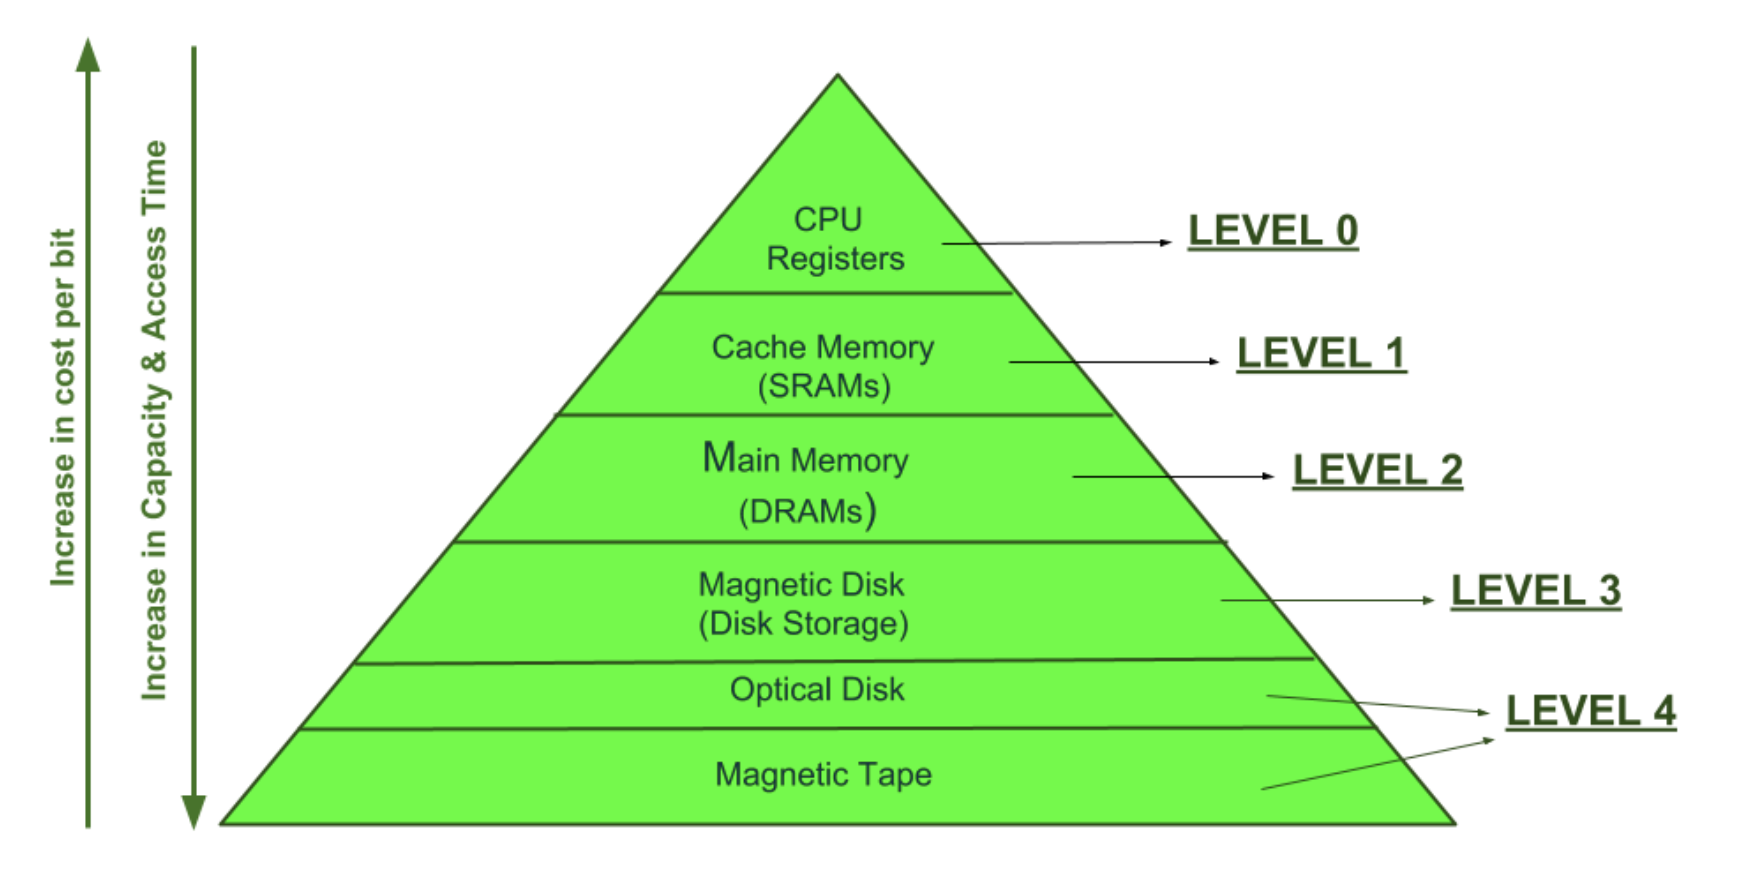
\includegraphics[width=0.6\textwidth]{Figures/herarchy.png}
        \end{center}
        \caption{Representation of the hierarchy of different types of memory in a system.}
        \label{}
    \end{figure}

\newpage
\subsection{Theoretical time}
% \addcontentsline{toc}{section}{Theoretical time}

    \paragraph*{}
    In this section, we discuss the concept of the "theoretical time of a CPU", which refers to the 
    estimated time required for a CPU to complete a given task under ideal conditions. This measure 
    assumes an optimal scenario, free from common real-world limitations such as memory latency, 
    system bottlenecks, or the complexities introduced by parallel execution. By focusing on theoretical 
    performance, we gain insights into the maximum potential of a CPU, providing a useful benchmark 
    for evaluating its capabilities across various workloads.
    \par

    \paragraph*{}
    Theoretical time allows us to break down CPU performance into fundamental parameters, helping us 
    understand how different architectural features influence the speed of computation. This model is 
    particularly valuable for comparing CPUs across generations or architectures, as it highlights 
    the efficiency of vectorization, micro-operations, and core usage, among other factors. While 
    real-world performance is often constrained by a variety of external factors, theoretical models 
    like this one offer a clear, baseline perspective on the CPU's potential.
    \par

    The following equation provides a framework for estimating the theoretical time a CPU would need 
    to complete a specific set of operations:

    \begin{equation}
        t_{CPU}=\frac{N_{ops} \times S_{ops}}{V_{vectorization} \times GH_{z_{CPU}} \times M_{micro-ops} \times C_{CPU}}
        \label{eq:timetheoretical}
    \end{equation}


    Where the parameters are: 
    \begin{enumerate}
        \item \(V_{vectorization}\): Vectorization factor: 16 (512-bit)
        \item \(M_{micro-ops}\): Micro-operations factor: 4, 6 (AMD Zen 3) or even 8 (Apple Silicon)
        \item \(GH_{z_{CPU}}\): Clock speed of the CPU
        \item \(C_{CPU}\): Number of cores in the CPU
        \item \(S_{ops}\): Sequence of operations. For example, in the case of matrix multiplication, it would have a value of 4.
        \item \(N_{ops}\): Number of operations
    \end{enumerate}

\newpage
\subsection{Benchmark operation}
% \addcontentsline{toc}{subsection}{Benchmark operation}
\subsubsection{Different Matrix-Multiplication functions}

     \paragraph*{}
     In order to achieve theoretical times (those associated with the previous expression), we need to 
     choose which mathematical operator will be used in the benchmarks. To begin, a common operator 
     will be used: matrix multiplication.

     \paragraph{}
     The next point to address is which matrix multiplication function we will use; the options are 
     either Julia's native function, associated with the \textbf{*} operator (\texttt{matrix\_multiplication}), or manually 
     constructing a custom matrix multiplication function (\texttt{my\_matrix\_multiplication}, \texttt{my\_efficient\_matrix\_multiplication}). To compare which of these options performs better, the number 
     of GFLOPS (y-axis) will be plotted for different values of N, the dimension of the matrices to 
     be multiplied (x-axis).

\vspace*{0.5cm}

\begin{comment}
 \lstinputlisting[language=Julia]{./Code/cpu/dot_func_comparison-v2.jl}   
\end{comment}

\begin{lstlisting}[language=Julia]
import Pkg
Pkg.activate(".")
Pkg.add(["PGFPlotsX", "CPUTime", "Plots", "LinearAlgebra", "MKL"])
using CPUTime
using Plots
using LinearAlgebra, MKL
using PGFPlotsX
using CpuId

# CPU info
cpuid = cpuinfo()
string_cpuid = string(cpuid)

println("AVX support: ", occursin("256", string_cpuid))
println("AVX-512 support: ", occursin("512 bit", string_cpuid))

# Function to initialize random matrices
function matrix_initialization(N)
    A = rand(Float32, N, N)
    B = rand(Float32, N, N)
    return A, B
end

# Function to multiply matrices using the built-in Julia method
function matrix_multiplication(A, B)
   return A * B  
end

# Function to multiply matrices using a custom method (manual loop)
function my_matrix_multiplication(A, B)
  (N, M) = size(A)
  (M, L) = size(B)
  C = zeros(Float32, (N, L))

  for i in 1:N, j in 1:L
      for k in 1:M
        C[i, j] = C[i, j] + A[i, k] * B[k, j]
      end
  end
  return C
end

# Transposing B for efficient memory access
function my_efficient_matrix_multiplication(A, B)
  (N, M) = size(A)
  (M, L) = size(B)
  BT = transpose(B) 
  C = zeros(Float32, (N, L))

  for k in 1:M
      for j in 1:L, i in 1:N
          C[i, j] = C[i, j] + A[i, k] * BT[j, k]
      end
  end
  return C
end

# Function to time matrix multiplication and calculate performance
function time_matrix_multilication(N, N_cores, matmul, AVX_value)
  Theoretical_time = 1e9 / (4.5e9 * AVX_value * 2 * N_cores)
  Time = zeros(length(N))

  for (i, n) in enumerate(N)
   A, B = matrix_initialization(n)
   t1 = time_ns()
   matmul(A, B)
   t2 = time_ns()
   Time[i] = (t2 - t1) / (2 * n^3)
  end 
  return Time, Theoretical_time
end

function get_avx_value(string_cpuid)
  AVX_value = 0
  if occursin("256 bit", string_cpuid)
      AVX_value = 8
  elseif occursin("512 bit", string_cpuid)
      AVX_value = 16
  end
  return AVX_value
end

AVX_value = get_avx_value(string_cpuid)
BLAS.set_num_threads(8)
N_threads = BLAS.get_num_threads()
N_cores = div(N_threads, 2)
println("Threads =", N_threads) 
println("Cores =", N_cores)

# Precompilation: Run matrix multiplication once to warm up
time_matrix_multilication(2000, N_cores, matrix_multiplication, AVX_value)

# Set range for matrix dimensions
N = 10:100:2500
BLAS.set_num_threads(2 * N_cores)

# Time the built-in matrix multiplication and custom multiplication
Time, Theoretical_time = time_matrix_multilication(N, N_cores, matrix_multiplication, AVX_value)
Time2, _ = time_matrix_multilication(N, N_cores, my_matrix_multiplication, AVX_value)
Time3, _ = time_matrix_multilication(N, N_cores, my_efficient_matrix_multiplication, AVX_value)

# Calculate GFLOPS for each method
GFLOPS = 1 ./ Time
GFLOPS2 = 1 ./ Time2
GFLOPS3 = 1 ./ Time3

# Plotting code here (omitted for brevity)
\end{lstlisting}

\vspace*{1cm}

\paragraph{} The results of running this code are shown in the following two figures; in the first one (Figure \ref{fig:1-dotproductcomparison}) you can see the difference between the functions \texttt{my\_matrix\_multiplication} and 
\texttt{my\_efficient\_matrix\_multiplication}. This difference lies in the transpose of the B matrix. 
This is because in Julia matrices are stored in column order, that is, consecutive columns are stored 
contiguously in memory. Therefore, when iterating over the elements of a matrix, it is more efficient 
to traverse it by columns than by rows.

\begin{figure}[h]
     \begin{center}
         % Recommended preamble:
\begin{tikzpicture}
\begin{axis}[width={15cm}, height={10cm}, xlabel={Matrix dimension [N]}, ylabel={FLOPS [GFLOPS]}, title={Comparison of different matrix multiplication functions}, legend={north east}, ymax={10},    scaled ticks=false,   % Prevents scientific notation or compression in the ticks
    xticklabel style={/pgf/number format/fixed},  % Ensures tick labels are printed in a fixed format without rounding
    xticklabel style={/pgf/number format/precision=0},  % Rounds the numbers to integers to avoid crowding
    ticklabel style = {font=\small},  % Reduces the size of the tick labels to prevent overlap
    ]
    \addplot[no marks, blue]
        table[row sep={\\}]
        {
            \\
            0.0  0.0023079523961738765  \\
            100.0  8.194097294901313  \\
            200.0  33.72498893859692  \\
            300.0  63.67891003491642  \\
            400.0  83.20933205921395  \\
            500.0  121.0965154318156  \\
            600.0  114.15410635879024  \\
            700.0  148.78480554332117  \\
            800.0  128.77979771936313  \\
            900.0  46.69649114974178  \\
            1000.0  149.39668260804913  \\
            1100.0  185.67318648613312  \\
            1200.0  139.70476585037548  \\
            1300.0  140.825722756572  \\
            1400.0  157.08443564188434  \\
            1500.0  189.98083748640684  \\
            1600.0  201.73749401185015  \\
            1700.0  238.16347699049706  \\
            1800.0  184.7190920582196  \\
            1900.0  236.60746961674465  \\
            2000.0  189.07665556113673  \\
            2100.0  208.35783211953395  \\
            2200.0  211.28693733594844  \\
            2300.0  220.6979894130633  \\
            2400.0  185.3414228183199  \\
        }
        ;
    \addplot[no marks, orange]
        table[row sep={\\}]
        {
            \\
            0.0  1.0689470871191875  \\
            100.0  1.7891119566042895  \\
            200.0  1.6363952973381144  \\
            300.0  1.833138380472606  \\
            400.0  1.8019750452823982  \\
            500.0  1.8633233611285047  \\
            600.0  1.829149502012656  \\
            700.0  1.814902720882529  \\
            800.0  1.691969911709576  \\
            900.0  1.67758644720142  \\
            1000.0  1.649210445467428  \\
            1100.0  1.4844659134712057  \\
            1200.0  1.50570400213252  \\
            1300.0  1.36048195288819  \\
            1400.0  1.441815509625949  \\
            1500.0  0.8870844660154257  \\
            1600.0  0.7907230876381947  \\
            1700.0  0.6699917469778933  \\
            1800.0  0.622945715952708  \\
            1900.0  0.4545396698327844  \\
            2000.0  0.5141040422999137  \\
            2100.0  0.5125469619014145  \\
            2200.0  0.49265788054693666  \\
            2300.0  0.497771062036038  \\
            2400.0  0.5078183160369875  \\
        }
        ;
    \addplot[no marks, green]
        table[row sep={\\}]
        {
            \\
            0.0  1.017293997965412  \\
            100.0  1.5855298659744814  \\
            200.0  1.9699571431686191  \\
            300.0  2.4009089137903974  \\
            400.0  2.424738077028364  \\
            500.0  2.4250974800940805  \\
            600.0  2.3888349809526823  \\
            700.0  2.3969416901613645  \\
            800.0  2.3114564185518116  \\
            900.0  2.2665805230657363  \\
            1000.0  2.1183366990174863  \\
            1100.0  2.098103432813833  \\
            1200.0  2.02596145383276  \\
            1300.0  1.9715949457443354  \\
            1400.0  2.010909758662662  \\
            1500.0  2.065411932336678  \\
            1600.0  1.9941957000538721  \\
            1700.0  1.9348035190308683  \\
            1800.0  1.86114085663287  \\
            1900.0  1.9272390772083445  \\
            2000.0  1.9553976471457613  \\
            2100.0  1.993427896663581  \\
            2200.0  1.9556294361633033  \\
            2300.0  1.9104629902084065  \\
            2400.0  1.9020792743764794  \\
        }
        ;
    \addplot[no marks, red]
        table[row sep={\\}]
        {
            \\
            0.0  288.0  \\
            100.0  288.0  \\
            200.0  288.0  \\
            300.0  288.0  \\
            400.0  288.0  \\
            500.0  288.0  \\
            600.0  288.0  \\
            700.0  288.0  \\
            800.0  288.0  \\
            900.0  288.0  \\
            1000.0  288.0  \\
            1100.0  288.0  \\
            1200.0  288.0  \\
            1300.0  288.0  \\
            1400.0  288.0  \\
            1500.0  288.0  \\
            1600.0  288.0  \\
            1700.0  288.0  \\
            1800.0  288.0  \\
            1900.0  288.0  \\
            2000.0  288.0  \\
            2100.0  288.0  \\
            2200.0  288.0  \\
            2300.0  288.0  \\
            2400.0  288.0  \\
        }
        ;
    \addlegendentry {\texttt{matrix\_multiplication}}
    \addlegendentry {\texttt{my\_efficient\_multiplication}}
    \addlegendentry {\texttt{my\_efficient\_matrix\_multiplication}}
\end{axis}
\end{tikzpicture}

     \end{center}
     \caption{Matrix product efficiency, tested on a Intel(R) Core(TM) i7-8557U CPU @ 1.70GHz (1)}
     \label{fig:1-dotproductcomparison}
 \end{figure}
 

\paragraph{} Now, by changing the dimension of the y-axis, we can see the comparison with the function \texttt{matrix\_multiplication} 
in Figure \ref{fig:2-dotproductcomparison}. This clearly shows the level of optimization that Julia's built-in dot product has. 
The theoretical GFLOPS value is also represented in this graph, and the convergence of the \texttt{matrix\_multiplication} function to 
this value can be observed. It can therefore be said that, seemingly quickly, we have achieved our objective: to observe 
convergence to theoretical values in experimental tests.

\begin{figure}[h]
     \begin{center}
        % Recommended preamble:
\begin{tikzpicture}
\begin{axis}[width={15cm}, height={10cm}, xlabel={Matrix dimension [N]}, ylabel={FLOPS [GFLOPS]}, title={Comparison of different matrix multiplication functions}, legend={north east}, ymax={10},    scaled ticks=false,   % Prevents scientific notation or compression in the ticks
    xticklabel style={/pgf/number format/fixed},  % Ensures tick labels are printed in a fixed format without rounding
    xticklabel style={/pgf/number format/precision=0},  % Rounds the numbers to integers to avoid crowding
    ticklabel style = {font=\small},  % Reduces the size of the tick labels to prevent overlap
    ]
    \addplot[no marks, blue]
        table[row sep={\\}]
        {
            \\
            10.0  0.0023079523961738765  \\
            110.0  8.194097294901313  \\
            210.0  33.72498893859692  \\
            310.0  63.67891003491642  \\
            410.0  83.20933205921395  \\
            510.0  121.0965154318156  \\
            610.0  114.15410635879024  \\
            710.0  148.78480554332117  \\
            810.0  128.77979771936313  \\
            910.0  46.69649114974178  \\
            1010.0  149.39668260804913  \\
            1110.0  185.67318648613312  \\
            1210.0  139.70476585037548  \\
            1310.0  140.825722756572  \\
            1410.0  157.08443564188434  \\
            1510.0  189.98083748640684  \\
            1610.0  201.73749401185015  \\
            1710.0  238.16347699049706  \\
            1810.0  184.7190920582196  \\
            1910.0  236.60746961674465  \\
            2010.0  189.07665556113673  \\
            2110.0  208.35783211953395  \\
            2210.0  211.28693733594844  \\
            2310.0  220.6979894130633  \\
            2410.0  185.3414228183199  \\
        }
        ;
    \addplot[no marks, orange]
        table[row sep={\\}]
        {
            \\
            10.0  1.0689470871191875  \\
            110.0  1.7891119566042895  \\
            210.0  1.6363952973381144  \\
            310.0  1.833138380472606  \\
            410.0  1.8019750452823982  \\
            510.0  1.8633233611285047  \\
            610.0  1.829149502012656  \\
            710.0  1.814902720882529  \\
            810.0  1.691969911709576  \\
            910.0  1.67758644720142  \\
            1010.0  1.649210445467428  \\
            1110.0  1.4844659134712057  \\
            1210.0  1.50570400213252  \\
            1310.0  1.36048195288819  \\
            1410.0  1.441815509625949  \\
            1510.0  0.8870844660154257  \\
            1610.0  0.7907230876381947  \\
            1710.0  0.6699917469778933  \\
            1810.0  0.622945715952708  \\
            1910.0  0.4545396698327844  \\
            2010.0  0.5141040422999137  \\
            2110.0  0.5125469619014145  \\
            2210.0  0.49265788054693666  \\
            2310.0  0.497771062036038  \\
            2410.0  0.5078183160369875  \\
        }
        ;
    \addplot[no marks, green]
        table[row sep={\\}]
        {
            \\
            10.0  1.017293997965412  \\
            110.0  1.5855298659744814  \\
            210.0  1.9699571431686191  \\
            310.0  2.4009089137903974  \\
            410.0  2.424738077028364  \\
            510.0  2.4250974800940805  \\
            610.0  2.3888349809526823  \\
            710.0  2.3969416901613645  \\
            810.0  2.3114564185518116  \\
            910.0  2.2665805230657363  \\
            1010.0  2.1183366990174863  \\
            1110.0  2.098103432813833  \\
            1210.0  2.02596145383276  \\
            1310.0  1.9715949457443354  \\
            1410.0  2.010909758662662  \\
            1510.0  2.065411932336678  \\
            1610.0  1.9941957000538721  \\
            1710.0  1.9348035190308683  \\
            1810.0  1.86114085663287  \\
            1910.0  1.9272390772083445  \\
            2010.0  1.9553976471457613  \\
            2110.0  1.993427896663581  \\
            2210.0  1.9556294361633033  \\
            2310.0  1.9104629902084065  \\
            2410.0  1.9020792743764794  \\
        }
        ;
    \addplot[no marks, red]
        table[row sep={\\}]
        {
            \\
            10.0  288.0  \\
            110.0  288.0  \\
            210.0  288.0  \\
            310.0  288.0  \\
            410.0  288.0  \\
            510.0  288.0  \\
            610.0  288.0  \\
            710.0  288.0  \\
            810.0  288.0  \\
            910.0  288.0  \\
            1010.0  288.0  \\
            1110.0  288.0  \\
            1210.0  288.0  \\
            1310.0  288.0  \\
            1410.0  288.0  \\
            1510.0  288.0  \\
            1610.0  288.0  \\
            1710.0  288.0  \\
            1810.0  288.0  \\
            1910.0  288.0  \\
            2010.0  288.0  \\
            2110.0  288.0  \\
            2210.0  288.0  \\
            2310.0  288.0  \\
            2410.0  288.0  \\
        }
        ;
        \addlegendentry {\texttt{matrix\_multiplication}}
        \addlegendentry {\texttt{my\_efficient\_multiplication}}
        \addlegendentry {\texttt{my\_efficient\_matrix\_multiplication}}
        \addlegendentry {Theoretical GFLOPS}        
\end{axis}
\end{tikzpicture}

     \end{center}
     \caption{Matrix product efficiency, tested on a Intel(R) Core(TM) i7-8557U CPU @ 1.70GHz (2)}
     \label{fig:2-dotproductcomparison}
 \end{figure}

\clearpage
\newpage


\subsubsection{Comparison of BLAS Operations Across Different Levels}
But what about matrix-vector multiplications? It is logical to consider the optimal shape and dimensions of these matrices. 
One might intuitively assume that a matrix-vector multiplication is faster than a matrix-matrix multiplication.
To visualize the load that the CPU experiences in both cases, the following code is used to plot the figures.

\vspace*{0.5cm}

\begin{comment}
\lstinputlisting[language=Julia]{../code/cpu/BLAS_levels.jl}  
\end{comment}

\begin{lstlisting}[language=Julia]
import Pkg
Pkg.activate(".")
Pkg.add(["CPUTime", "Plots", "LinearAlgebra", "MKL", "PGFPlotsX", "CpuId"])
using CPUTime, Plots, LinearAlgebra, MKL, PGFPlotsX, CpuId

cpuid = cpuinfo() # CPU Features
string_cpuid = string(cpuid)
println("AVX support: ", occursin("256", string_cpuid))
println("AVX-512 support: ", occursin("512 bit", string_cpuid))

function matrix_initialization(N) 
  A = rand(Float32, N, N )
  B = rand(Float32, N, N )
  return A, B 
end 

function matrix_vector_initialization(N)
    A = rand(Float32, N, N )
    B = rand(Float32, N, 1 )
    return A, B 
end 

function vector_vector_initialization(N)
    A = rand(Float32, N, 1 )
    B = rand(Float32, N, 1 )
    return A, B 
end 

function vector_multiplication(A, B)
    return dot(A, B)  
end

function matrix_multiplication(A, B)
    return A * B  
end

function time_matrix_multiplication(N, N_cores, matinit, matmul, AVX_value)
    Time = zeros(length(N))
    Theoretical_time = 1e9 / (4.5e9 * AVX_value * 2 * N_cores)

    for (i, n) in enumerate(N)  
     A, B = matinit(n)
     t1 = time_ns()
     matmul(A, B)
     t2 = time_ns()
     dt = t2 - t1
     Time[i] = dt / (2 * n^3)
     println("N=", n, " Time per operation =", Time[i], " nsec")
     println("N=", n, " Theoretical time per operation =", Theoretical_time, " nsec")
    end 

    return Time, Theoretical_time
end

function get_avx_value(string_cpuid)
    AVX_value = 0
    if occursin("256 bit", string_cpuid)
        AVX_value = 8
    elseif occursin("512 bit", string_cpuid)
        AVX_value = 16
    else
        AVX_value = 0
    end
    return AVX_value
end

AVX_value = get_avx_value(string_cpuid)

N_cores = 4
N = Vector([10:25:2500; 2500:100:5000])
BLAS.set_num_threads(2 * N_cores)
println("Threads = ", BLAS.get_num_threads(), " N_cores =", N_cores)

Time, Theoretical_time = time_matrix_multiplication(N, N_cores, matrix_initialization, matrix_multiplication, AVX_value)
\end{lstlisting}

\vspace*{0.5cm}

\begin{figure}[h]
\begin{center}
    % Recommended preamble:
\begin{tikzpicture}
\begin{axis}[width={15cm}, height={10cm}, xlabel={Matrix dimension [N]}, ylabel={FLOPS [GFLOPS]}, title={Comparison of Matrix-Vector Multiplication and Matrix-Matrix Multiplication}, legend={north east}, ymax={500}]
    \addplot[no marks, blue]
        table[row sep={\\}]
        {
            \\
            10.0  0.00023735286051140286  \\
            35.0  1.8266445126107702  \\
            60.0  28.92728003214142  \\
            85.0  1.6462358731316078  \\
            110.0  8.66341869827415  \\
            135.0  19.369447385719965  \\
            160.0  18.755136943178254  \\
            185.0  24.092712207836684  \\
            210.0  36.257857141458885  \\
            235.0  44.314565420784135  \\
            260.0  58.44075957027288  \\
            285.0  54.576140719819314  \\
            310.0  54.29418111303892  \\
            335.0  78.69009868868586  \\
            360.0  89.8249072746893  \\
            385.0  78.31813287970999  \\
            410.0  91.11580873361176  \\
            435.0  82.77338472592267  \\
            460.0  109.91630591956493  \\
            485.0  83.6076671790578  \\
            510.0  116.31012526150948  \\
            535.0  136.3508365303236  \\
            560.0  104.29141449863026  \\
            585.0  140.48561525288082  \\
            610.0  134.55378496801708  \\
            635.0  116.21255795925332  \\
            660.0  129.30891407336844  \\
            685.0  114.43687076149929  \\
            710.0  143.64748649708972  \\
            735.0  135.7695713208871  \\
            760.0  125.21616301012152  \\
            785.0  142.40380890308208  \\
            810.0  146.4390285839937  \\
            835.0  151.08798486895742  \\
            860.0  136.79613589241458  \\
            885.0  151.83550320744158  \\
            910.0  184.10195477821713  \\
            935.0  183.68331047779773  \\
            960.0  165.89797980034737  \\
            985.0  186.63288902307468  \\
            1010.0  145.5539478662233  \\
            1035.0  85.84116813955796  \\
            1060.0  180.31715559942725  \\
            1085.0  166.8072682514341  \\
            1110.0  156.5568485028589  \\
            1135.0  188.11624237215517  \\
            1160.0  104.95485127794238  \\
            1185.0  125.42631303170059  \\
            1210.0  143.3921637808318  \\
            1235.0  175.4632141674464  \\
            1260.0  162.0556196725115  \\
            1285.0  226.89372516272846  \\
            1310.0  201.79996849247254  \\
            1335.0  196.53080970413205  \\
            1360.0  120.54266472715214  \\
            1385.0  194.33739426070323  \\
            1410.0  190.50246449503956  \\
            1435.0  149.27629620095067  \\
            1460.0  168.48990456887893  \\
            1485.0  203.62494767542074  \\
            1510.0  217.84711470582596  \\
            1535.0  219.56858219147125  \\
            1560.0  206.84355955322113  \\
            1585.0  160.34243896137565  \\
            1610.0  197.72951864087614  \\
            1635.0  189.9645287963804  \\
            1660.0  143.88657212456386  \\
            1685.0  145.95230940426606  \\
            1710.0  182.71589356195926  \\
            1735.0  225.33715315261833  \\
            1760.0  226.5185839605248  \\
            1785.0  170.93730928923088  \\
            1810.0  225.17261440412383  \\
            1835.0  201.19296185498513  \\
            1860.0  187.86489412050884  \\
            1885.0  215.16034520656507  \\
            1910.0  211.9352634672822  \\
            1935.0  154.12981763154013  \\
            1960.0  228.4821628792833  \\
            1985.0  205.25343700293823  \\
            2010.0  157.60220556890428  \\
            2035.0  233.90041455368387  \\
            2060.0  182.87409933734776  \\
            2085.0  211.02988778492522  \\
            2110.0  188.1566760543063  \\
            2135.0  244.26527954650308  \\
            2160.0  265.7174692898608  \\
            2185.0  156.5263302218174  \\
            2210.0  268.2479682949384  \\
            2235.0  242.02406286743764  \\
            2260.0  293.40068847583615  \\
            2285.0  201.2885254632914  \\
            2310.0  278.15430681461964  \\
            2335.0  276.62191232583945  \\
            2360.0  238.34265072537647  \\
            2385.0  278.18471215461506  \\
            2410.0  229.24491546677055  \\
            2435.0  276.83255957868005  \\
            2460.0  269.43063227706887  \\
            2485.0  246.2499101261397  \\
            2500.0  274.7579123420797  \\
            2600.0  199.8495783982345  \\
            2700.0  242.49924205896602  \\
            2800.0  245.01651263628966  \\
            2900.0  223.6033542556816  \\
            3000.0  196.72210624705218  \\
            3100.0  222.71242812611638  \\
            3200.0  235.508416371348  \\
            3300.0  249.4599823414236  \\
            3400.0  256.6880799584675  \\
            3500.0  251.92273749687772  \\
            3600.0  268.19559000362557  \\
            3700.0  239.8471743599322  \\
            3800.0  193.3464055099314  \\
            3900.0  225.37951408805193  \\
            4000.0  244.35539841008978  \\
            4100.0  239.66615698125284  \\
            4200.0  256.69404704164407  \\
            4300.0  258.0059741848452  \\
            4400.0  237.78058288125905  \\
            4500.0  257.3327020518556  \\
            4600.0  246.76345865474775  \\
            4700.0  261.37674684881256  \\
            4800.0  267.80212423297974  \\
            4900.0  262.4908914161355  \\
            5000.0  259.8166895771811  \\
        }
        ;
    \addplot[no marks, red]
        table[row sep={\\}]
        {
            \\
            10.0  0.04038772213247173  \\
            35.0  0.6474630021141649  \\
            60.0  1.9072847682119205  \\
            85.0  3.369869402985075  \\
            110.0  3.6309077269317327  \\
            135.0  3.977520733304234  \\
            160.0  4.690792487402657  \\
            185.0  3.826373749231371  \\
            210.0  3.871987356775978  \\
            235.0  4.203615604186489  \\
            260.0  4.292472298949106  \\
            285.0  3.9647093278664514  \\
            310.0  4.018398494668618  \\
            335.0  4.833326155303847  \\
            360.0  5.184518451845184  \\
            385.0  4.729805191697114  \\
            410.0  4.763591538319849  \\
            435.0  4.552343834578327  \\
            460.0  4.951039460907612  \\
            485.0  2.34843379508299  \\
            510.0  4.421514296399551  \\
            535.0  1.3554534239731395  \\
            560.0  1.1552835989147112  \\
            585.0  1.8188509974515623  \\
            610.0  2.08815012682664  \\
            635.0  2.189007326096811  \\
            660.0  1.939214787180526  \\
            685.0  2.1015281398077734  \\
            710.0  2.5428837340691435  \\
            735.0  2.7973250069904  \\
            760.0  2.7996568287682186  \\
            785.0  2.9174626395763648  \\
            810.0  2.8470075178182057  \\
            835.0  1.471997787437798  \\
            860.0  3.8074450067181123  \\
            885.0  3.0598013458476983  \\
            910.0  1.7348021506435067  \\
            935.0  0.11851605923274638  \\
            960.0  4.204955057717753  \\
            985.0  4.164529442189777  \\
            1010.0  1.914215881743079  \\
            1035.0  3.756292045592018  \\
            1060.0  4.3230182639441965  \\
            1085.0  4.153626583774667  \\
            1110.0  3.9032379673130353  \\
            1135.0  4.476096330450555  \\
            1160.0  1.2727755985762619  \\
            1185.0  3.9994218286733103  \\
            1210.0  4.445929018789144  \\
            1235.0  3.4416056952992347  \\
            1260.0  5.430356431274831  \\
            1285.0  1.7928269549709968  \\
            1310.0  4.532877958844606  \\
            1335.0  3.1668770839978286  \\
            1360.0  4.668967998031037  \\
            1385.0  3.2287724276998873  \\
            1410.0  4.963270400998596  \\
            1435.0  4.711894230791232  \\
            1460.0  6.246025908876471  \\
            1485.0  4.715581106669247  \\
            1510.0  5.15222112001663  \\
            1535.0  3.754623115497815  \\
            1560.0  2.3816490884339894  \\
            1585.0  5.914861406396048  \\
            1610.0  5.3791456162795885  \\
            1635.0  6.012496302952128  \\
            1660.0  6.007942711314167  \\
            1685.0  6.9813860850535425  \\
            1710.0  6.123596505648531  \\
            1735.0  7.2196999131782045  \\
            1760.0  5.33927658800645  \\
            1785.0  3.832358772937952  \\
            1810.0  6.435296405497728  \\
            1835.0  7.2067516779672625  \\
            1860.0  6.040874910620509  \\
            1885.0  7.117132816357352  \\
            1910.0  4.81206359716956  \\
            1935.0  2.8951521487325964  \\
            1960.0  4.562245447522479  \\
            1985.0  5.953773252765552  \\
            2010.0  6.166481727671097  \\
            2035.0  7.578540043664366  \\
            2060.0  3.0203590964687863  \\
            2085.0  6.945680464107853  \\
            2110.0  6.1668645134838265  \\
            2135.0  6.675974196685465  \\
            2160.0  6.568251760459282  \\
            2185.0  4.150951352516885  \\
            2210.0  3.761134354609798  \\
            2235.0  2.9333378354175044  \\
            2260.0  3.48676624890006  \\
            2285.0  3.7088714641241993  \\
            2310.0  2.083170263379853  \\
            2335.0  3.720556900437243  \\
            2360.0  3.86289684665799  \\
            2385.0  4.510773327539133  \\
            2410.0  3.4254466553961507  \\
            2435.0  1.9768722393521678  \\
            2460.0  4.487940828240002  \\
            2485.0  3.5444291639354986  \\
            2500.0  3.7150182734318835  \\
            2600.0  3.960732501149843  \\
            2700.0  3.8824020938343033  \\
            2800.0  5.553367579100072  \\
            2900.0  2.5307553733037205  \\
            3000.0  3.672333962050509  \\
            3100.0  4.267501752961828  \\
            3200.0  5.159863817891072  \\
            3300.0  3.6895337008750357  \\
            3400.0  5.682082099696456  \\
            3500.0  5.527524363973717  \\
            3600.0  5.382689047743746  \\
            3700.0  5.019562176114034  \\
            3800.0  4.976975456858946  \\
            3900.0  3.2288561665580295  \\
            4000.0  4.355687629683794  \\
            4100.0  5.800819326908262  \\
            4200.0  6.761830616143066  \\
            4300.0  6.065022353494366  \\
            4400.0  7.012545247850552  \\
            4500.0  6.178148514147655  \\
            4600.0  6.6362328276498825  \\
            4700.0  6.034111990550837  \\
            4800.0  5.080672209979948  \\
            4900.0  4.090876060000765  \\
            5000.0  4.679102035400027  \\
        }
        ;
    \addplot[no marks, green]
        table[row sep={\\}]
        {
            \\
            10.0  0.0032674399607907204  \\
            35.0  0.020958083832335328  \\
            60.0  0.046838407494145196  \\
            85.0  0.07834101382488479  \\
            110.0  0.08644400785854617  \\
            135.0  0.10424710424710423  \\
            160.0  0.14890646812470917  \\
            185.0  0.11824864173857462  \\
            210.0  0.1972757162987318  \\
            235.0  0.23653749370910923  \\
            260.0  0.47619047619047616  \\
            285.0  0.29290853031860226  \\
            310.0  0.38969201759899436  \\
            335.0  0.2571976967370442  \\
            360.0  0.23323615160349856  \\
            385.0  0.3389084507042253  \\
            410.0  0.4017638412542871  \\
            435.0  0.31487513572204123  \\
            460.0  0.46605876393110435  \\
            485.0  0.6123737373737373  \\
            510.0  0.07051991150442478  \\
            535.0  0.2859433458043827  \\
            560.0  0.3604763437399421  \\
            585.0  0.412407472682411  \\
            610.0  0.47470817120622566  \\
            635.0  0.4191419141914191  \\
            660.0  0.3880070546737214  \\
            685.0  0.430411561420044  \\
            710.0  0.46103896103896097  \\
            735.0  0.448444173276388  \\
            760.0  0.5594405594405594  \\
            785.0  0.5516514406184118  \\
            810.0  0.5465587044534412  \\
            835.0  0.5831005586592178  \\
            860.0  0.5041031652989448  \\
            885.0  0.22859356838434716  \\
            910.0  0.2720885035132307  \\
            935.0  0.3410541674265913  \\
            960.0  0.5010438413361169  \\
            985.0  0.5093071354705274  \\
            1010.0  0.618304254667891  \\
            1035.0  0.5569007263922517  \\
            1060.0  0.6257378984651712  \\
            1085.0  0.8420644159875824  \\
            1110.0  0.847651775486827  \\
            1135.0  0.8657513348588863  \\
            1160.0  0.4597701149425288  \\
            1185.0  0.484167517875383  \\
            1210.0  0.46772323154232703  \\
            1235.0  0.4209988068859724  \\
            1260.0  0.4190919674039581  \\
            1285.0  0.35585710329548603  \\
            1310.0  0.5059868675164156  \\
            1335.0  0.5519950382468473  \\
            1360.0  0.690180157320477  \\
            1385.0  0.35259674134419555  \\
            1410.0  0.5380652547223812  \\
            1435.0  0.5948186528497409  \\
            1460.0  0.5394420838721596  \\
            1485.0  0.4638450726222083  \\
            1510.0  0.4946764946764947  \\
            1535.0  0.5824321760576741  \\
            1560.0  0.6439628482972136  \\
            1585.0  0.3203314470493128  \\
            1610.0  0.5905006418485237  \\
            1635.0  0.31202290076335876  \\
            1660.0  0.31907736665064873  \\
            1685.0  0.4763250883392226  \\
            1710.0  0.0909526089037817  \\
            1735.0  0.4149724946185123  \\
            1760.0  0.44915146101824677  \\
            1785.0  0.4031620553359684  \\
            1810.0  0.6237077877325983  \\
            1835.0  0.6719150494324423  \\
            1860.0  0.7993124194241513  \\
            1885.0  0.8176100628930817  \\
            1910.0  0.5247252747252747  \\
            1935.0  0.6116642958748222  \\
            1960.0  0.920836269673479  \\
            1985.0  0.7245847782442052  \\
            2010.0  0.7545045045045046  \\
            2035.0  0.7394622093023255  \\
            2060.0  0.6646233263429585  \\
            2085.0  0.5122850122850122  \\
            2110.0  0.46573225913254607  \\
            2135.0  0.3538869550803912  \\
            2160.0  0.8121827411167513  \\
            2185.0  0.34918098282061527  \\
            2210.0  0.4482758620689655  \\
            2235.0  0.45926230350354463  \\
            2260.0  0.6781695423855965  \\
            2285.0  0.5805386178861789  \\
            2310.0  0.6193029490616622  \\
            2335.0  0.182486030245008  \\
            2360.0  0.6398264877321405  \\
            2385.0  0.6531562371628098  \\
            2410.0  0.8423628102062216  \\
            2435.0  0.7975761546020308  \\
            2460.0  0.09568447461055252  \\
            2485.0  0.8577839143942009  \\
            2500.0  0.8305647840531561  \\
            2600.0  0.9967414222733372  \\
            2700.0  0.8478568064060291  \\
            2800.0  0.9362982778799532  \\
            2900.0  0.821297082979326  \\
            3000.0  0.5694760820045558  \\
            3100.0  0.6203722233340004  \\
            3200.0  0.67425200168563  \\
            3300.0  0.7806031933767003  \\
            3400.0  0.6726679196755366  \\
            3500.0  0.6440334897414666  \\
            3600.0  0.23203351595230426  \\
            3700.0  0.5489614243323442  \\
            3800.0  0.5302078973071019  \\
            3900.0  0.6821163095758637  \\
            4000.0  0.887606790191945  \\
            4100.0  0.8935381933093604  \\
            4200.0  0.9595613433858808  \\
            4300.0  0.7872574148663494  \\
            4400.0  0.7692980155608008  \\
            4500.0  0.9266886326194399  \\
            4600.0  0.9240658899156288  \\
            4700.0  0.2673340538080883  \\
            4800.0  0.9374084562054488  \\
            4900.0  0.9862131427996377  \\
            5000.0  0.7254788160185722  \\
        }
        ;
    \addplot[no marks, orange]
        table[row sep={\\}]
        {
            \\
            10.0  288.0  \\
            35.0  288.0  \\
            60.0  288.0  \\
            85.0  288.0  \\
            110.0  288.0  \\
            135.0  288.0  \\
            160.0  288.0  \\
            185.0  288.0  \\
            210.0  288.0  \\
            235.0  288.0  \\
            260.0  288.0  \\
            285.0  288.0  \\
            310.0  288.0  \\
            335.0  288.0  \\
            360.0  288.0  \\
            385.0  288.0  \\
            410.0  288.0  \\
            435.0  288.0  \\
            460.0  288.0  \\
            485.0  288.0  \\
            510.0  288.0  \\
            535.0  288.0  \\
            560.0  288.0  \\
            585.0  288.0  \\
            610.0  288.0  \\
            635.0  288.0  \\
            660.0  288.0  \\
            685.0  288.0  \\
            710.0  288.0  \\
            735.0  288.0  \\
            760.0  288.0  \\
            785.0  288.0  \\
            810.0  288.0  \\
            835.0  288.0  \\
            860.0  288.0  \\
            885.0  288.0  \\
            910.0  288.0  \\
            935.0  288.0  \\
            960.0  288.0  \\
            985.0  288.0  \\
            1010.0  288.0  \\
            1035.0  288.0  \\
            1060.0  288.0  \\
            1085.0  288.0  \\
            1110.0  288.0  \\
            1135.0  288.0  \\
            1160.0  288.0  \\
            1185.0  288.0  \\
            1210.0  288.0  \\
            1235.0  288.0  \\
            1260.0  288.0  \\
            1285.0  288.0  \\
            1310.0  288.0  \\
            1335.0  288.0  \\
            1360.0  288.0  \\
            1385.0  288.0  \\
            1410.0  288.0  \\
            1435.0  288.0  \\
            1460.0  288.0  \\
            1485.0  288.0  \\
            1510.0  288.0  \\
            1535.0  288.0  \\
            1560.0  288.0  \\
            1585.0  288.0  \\
            1610.0  288.0  \\
            1635.0  288.0  \\
            1660.0  288.0  \\
            1685.0  288.0  \\
            1710.0  288.0  \\
            1735.0  288.0  \\
            1760.0  288.0  \\
            1785.0  288.0  \\
            1810.0  288.0  \\
            1835.0  288.0  \\
            1860.0  288.0  \\
            1885.0  288.0  \\
            1910.0  288.0  \\
            1935.0  288.0  \\
            1960.0  288.0  \\
            1985.0  288.0  \\
            2010.0  288.0  \\
            2035.0  288.0  \\
            2060.0  288.0  \\
            2085.0  288.0  \\
            2110.0  288.0  \\
            2135.0  288.0  \\
            2160.0  288.0  \\
            2185.0  288.0  \\
            2210.0  288.0  \\
            2235.0  288.0  \\
            2260.0  288.0  \\
            2285.0  288.0  \\
            2310.0  288.0  \\
            2335.0  288.0  \\
            2360.0  288.0  \\
            2385.0  288.0  \\
            2410.0  288.0  \\
            2435.0  288.0  \\
            2460.0  288.0  \\
            2485.0  288.0  \\
            2500.0  288.0  \\
            2600.0  288.0  \\
            2700.0  288.0  \\
            2800.0  288.0  \\
            2900.0  288.0  \\
            3000.0  288.0  \\
            3100.0  288.0  \\
            3200.0  288.0  \\
            3300.0  288.0  \\
            3400.0  288.0  \\
            3500.0  288.0  \\
            3600.0  288.0  \\
            3700.0  288.0  \\
            3800.0  288.0  \\
            3900.0  288.0  \\
            4000.0  288.0  \\
            4100.0  288.0  \\
            4200.0  288.0  \\
            4300.0  288.0  \\
            4400.0  288.0  \\
            4500.0  288.0  \\
            4600.0  288.0  \\
            4700.0  288.0  \\
            4800.0  288.0  \\
            4900.0  288.0  \\
            5000.0  288.0  \\
        }
        ;
    \addlegendentry {\texttt{matrix\_multiplication}}
    \addlegendentry {\texttt{matrix\_vector\_multiplication}}
    \addlegendentry {{\texttt{vector\_vector\_multiplication}}}
    \addlegendentry {Theoretical time}
\end{axis}
\end{tikzpicture}

\end{center}
    \caption{Representation of GFLOPS for the different levels of BLAS: matrix multiplication (Level 3 BLAS), 
    matrix-vector multiplication (Level 2 BLAS), and vector multiplication (dot product, Level 1 BLAS).}
    \label{fig:matvec_vs_matmul}
\end{figure}

\newpage

\paragraph*{} Figure \ref{fig:matvec_vs_matmul} illustrates the inherent limitation in matrix-vector multiplication 
(which is not due to CPU capacity but rather a bottleneck issue). This limitation arises because the ``usability'' of data in a matrix-matrix operation is higher than in a matrix-vector operation. 
Consider the following example with $N$:

\begin{equation}
    \begin{bmatrix}
        a_{11} & \hdots & a_{1N} \\
        \vdots & \ddots & \vdots \\
        a_{N1} & \hdots & a_{NN} 
    \end{bmatrix}
    \begin{bmatrix}
        b_{11} & \hdots & b_{1N} \\
        \vdots & \ddots & \vdots \\
        b_{N1} & \hdots & b_{NN} 
    \end{bmatrix}
    =
    \begin{bmatrix}
        c_{11} & \hdots & c_{1N} \\
        \vdots & \ddots & \vdots \\
        c_{N1} & \hdots & c_{NN} 
    \end{bmatrix}
    \label{eq_matrix1}
\end{equation}

\vspace{0.5cm}

\begin{equation}
    \begin{bmatrix}
        \alpha_{11} & \hdots & \alpha_{1N} \\
        \vdots & \ddots & \vdots \\
        \alpha_{N1} & \hdots & \alpha_{NN} 
    \end{bmatrix}
    \begin{bmatrix}
        \beta_{1} \\
        \vdots \\
        \beta_{N}
    \end{bmatrix}
    =
    \begin{bmatrix}
        \gamma_{1} \\
        \vdots \\
        \gamma_{N}
    \end{bmatrix}
    \label{eq_matrix2}
\end{equation}

\vspace{0.5cm}

\paragraph*{} In this example, vector $\vec{a}_1 = \sum_{i=1}^{N} a_{1i} \vec{e}_i$ is used $N$ times to compute $N$ values ($\sum_{i=1}^{N} c_{i1} \vec{e}_i$). 
In contrast, the vector of elements $\vec{\alpha}_1 = \sum_{i=1}^{N} \alpha_{1i} \vec{e}_i$ is only used once (to compute $\gamma_{1}$).

\paragraph*{} We can define the term "usability" as the ratio between the number of operations performed by the CPU and the number 
of data elements (in this case, Float32) used during the process. This can be expressed as:

\begin{equation}
    U = \frac{N_{ops}}{N_{data}}
\end{equation}

where $N_{ops}$ represents the number of operations executed by the CPU, and $N_{data}$ denotes the number of data elements 
involved in the process.

\paragraph*{} For matrix multiplication of dimension $N$, considering the use of Fused Multiply-Add (FMA), we have $N_{ops} = N^3$ 
and $N_{data} = 2N^2$. This yields a usability value greater than 1.

\paragraph*{} In the case of matrix-vector multiplication, again with dimension $N$ (as shown in expression \ref{eq_matrix2}),
$N_{ops} = N^2$ and $N_{data} = N^2 + N$. Here, the usability value is approximately 1.

\paragraph*{Scalar product} It is worth noting that the graph \ref{fig:matvec_vs_matmul} also includes the vector-vector product.
As expected, the results are even worse. The value of \textbf{U} is less than 1 ($N_{ops} = N$ and $N_{data} = 2N$)

\paragraph*{} In conclusion, \textbf{as the usability value tends towards infinity, and with sufficiently large values of N, the CPU's 
performance approaches its theoretical maximum.}

%!!! NOTE !!! For including .tex files that makes some graphics from a .jl file, use this:
% \begin{tikzpicture}
% \begin{axis}[xlabel={x}, ylabel={y}, title={Gráfico de ejemplo}]
%    \addplot[no marks]
%       table[row sep={\\}]
%       {
%           .
%           .
%           .
%        }
%       ;
% \end{axis}
% \end{tikzpicture}
\clearpage
\newpage
\section{GPU Performance: Benchmark Analysis}

\subsection{Understanding the GPU}

(Before starting, it is important to mention that during the study of this project, an NVIDIA GeForce RTX 3050 was used as the base graphics card. Therefore, unless explicitly mentioned in specific subsections, this graphics card will be assumed as the default.)

\subsubsection{Introduction to GPUs}

A GPU is a specialized electronic circuit designed to accelerate the creation and rendering of images, animations, and videos for display output. GPUs are highly efficient at performing parallel calculations on large blocks of data, making them essential not only for graphics tasks but also for computational workloads like machine learning and scientific simulations.

\begin{center}
\textbf{How is a GPU different from a CPU?}
\end{center}
GPUs differ from CPUs in their architecture and processing capabilities. GPUs have many small, simple cores designed for parallel processing, making them highly effective for tasks like image processing and deep learning, which require handling many operations simultaneously. In contrast, CPUs have fewer, more complex cores optimized for general-purpose tasks, including complex decision-making and single-threaded applications.

\begin{center}
\textbf{How is a GPU similar to a CPU?} 
\end{center}
Despite their differences, GPUs and CPUs both execute instructions and process data using semiconductor technology. They share fundamental principles of binary logic and data management. Additionally, both have evolved to handle a broader range of tasks: GPUs now support general-purpose computing, and CPUs include more cores and specialized instructions for parallel processing.

\subsubsection{Vectorization and parallelism}

As previously mentioned, GPUs support both vectorization and parallelization, though differently from CPUs. While CPUs have a few powerful cores optimized for sequential processing and use vectorization, GPUs consist of thousands of smaller cores designed for massive parallelism. This makes GPUs exceptionally efficient for tasks like matrix multiplication, where many operations can be performed concurrently.

\begin{center}
    \textbf{Vectorization:}    
\end{center}
GPUs achieve vectorization by executing the same instruction across multiple cores organized in grids and blocks (or threads in CUDA). Each core processes a different data set simultaneously, enabling efficient large-scale data processing.

\begin{center}
    \textbf{Parallelization:}    
\end{center}
GPUs excel in parallelization by leveraging their many cores to handle thousands of threads concurrently, making them ideal for tasks that can be divided into numerous parallel operations.
 
\subsubsection{Memory Access}

Memory access in GPUs is optimized for high throughput and parallel processing. GPUs use several types of memory with different characteristics:
\begin{itemize}
    \item \textbf{Global Memory:} This is the largest and slowest memory on the GPU, accessible by all cores. It's used for storing large datasets and is suitable for tasks that involve significant data exchange between the CPU and GPU. However, access to global memory can be slow if not managed efficiently.
    \item \textbf{Shared Memory:} Shared memory is much faster than global memory and is used for communication between threads within the same block. It allows for efficient data sharing and reduces the need to repeatedly access global memory, improving performance for tasks with high inter-thread communication.
    \item \textbf{Local Memory:} Each thread has its own local memory, which is private and used for storing data specific to that thread. Local memory helps in storing intermediate results and temporary data.
    \item \textbf{Texture and Constant Memory:} These are specialized types of memory. Texture memory is optimized for spatial locality and is used for image and graphical data, while constant memory is used for read-only data that remains constant across all threads during a kernel execution.
\end{itemize}
    Efficient memory access is crucial for performance, and optimizing memory use involves minimizing global memory accesses, maximizing shared memory usage, and ensuring coalesced memory accesses to reduce latency and improve throughput.
\subsection{GPU Hardware}
    The hardware architecture of GPUs is designed to facilitate massive parallel processing, making them ideal for tasks that can be parallelized. Key components include:

\begin{itemize}
    \item \textbf{Cores:} GPUs are equipped with thousands of small, simple cores designed for parallel execution. Unlike CPU cores, which are few in number but powerful, GPU cores are numerous and less complex. These cores work together to perform many operations simultaneously, which is crucial for tasks like rendering images and processing large datasets.
    \item  \textbf{Streaming Multiprocessors (SMs):} The GPU cores are organized into Streaming Multiprocessors (SMs). Each SM contains multiple cores, a portion of shared memory, and scheduling hardware. SMs manage the execution of threads within a block, handling the scheduling and synchronization necessary for efficient parallel processing.
    \item \textbf{Memory Hierarchy:} The GPU has a complex memory hierarchy designed to balance speed and capacity.
    \item  \textbf{Interconnects:} High-speed interconnects, such as NVIDIA’s NVLink and AMD's Infinity Fabric, are used to connect multiple GPUs or to facilitate rapid communication between different parts of a GPU. These interconnects enhance performance by allowing for efficient data transfer and coordination among multiple GPUs in a system.
\end{itemize}


\subsection{GPU Software}
    GPU software encompasses various tools and frameworks that facilitate the development and execution of parallel programs on GPUs. Major components include:

\begin{itemize}
    \item \textbf{CUDA:} NVIDIA’s Compute Unified Device Architecture (CUDA) is a parallel computing platform and API that allows developers to leverage NVIDIA GPUs for general-purpose computing. CUDA provides extensions to standard programming languages such as C, C++, and Fortran, and includes a comprehensive toolkit for developing GPU-accelerated applications. It supports features like kernel programming, memory management, and inter-thread synchronization.
    \item \textbf{OpenCL:} The Open Computing Language (OpenCL) is an open standard for parallel programming across heterogeneous systems, including GPUs from various vendors. OpenCL provides a unified programming model and API that enables developers to write code that can run on different types of processors (CPUs, GPUs, FPGAs) and is suitable for a wide range of applications.
    \item \textbf{Libraries and Frameworks:} Several libraries and frameworks provide pre-built functions and abstractions for GPU programming, making it easier to develop high-performance applications:
    \begin{enumerate}
        \item \textbf{cuBLAS:} A library for performing basic linear algebra operations on NVIDIA GPUs, optimized for performance.
        \item \textbf{cuDNN:} A library for deep neural network operations, providing highly optimized routines for deep learning tasks.
        \item \textbf{TensorFlow and PyTorch:} Popular machine learning frameworks that utilize GPU acceleration to improve training and inference performance.
    \end{enumerate}
    \item \textbf{Driver Software:} GPU drivers are essential for enabling communication between the operating system and GPU hardware. They handle the execution of GPU-accelerated applications, manage resources, and provide support for various APIs and frameworks. Regular updates to drivers ensure compatibility with new software and hardware features.
    \item \textbf{Development Tools:} Various development tools and IDEs (Integrated Development Environments) support GPU programming by providing debugging, profiling, and performance analysis capabilities. Examples include NVIDIA Nsight and AMD ROCm tools.
\end{itemize}
    
    Understanding these software components and their interaction with GPU hardware is crucial for developing efficient GPU-accelerated applications and achieving optimal performance.

\subsection{Operators Used in Benchmark.}
    \subsubsection{CUDA}
    Compute Unified Device Architecture (CUDA) is a parallel computing platform and programming model developed by NVIDIA. It enables developers to leverage NVIDIA GPUs for general-purpose computing tasks beyond traditional graphics rendering. CUDA provides a set of extensions to standard programming languages such as C, C++, and Fortran, allowing developers to write programs that execute on the GPU. CUDA facilitates efficient parallel processing by exposing low-level GPU architecture features, including fine-grained control over memory and execution.

    \paragraph{Key Features of CUDA:}
    \begin{itemize}
        \item \textbf{Parallel Computing Model:} CUDA allows for the execution of multiple threads in parallel on the GPU. Threads are organized into blocks, and blocks are organized into grids, providing a flexible and scalable way to manage parallelism.
        \item \textbf{Memory Hierarchy:} CUDA provides access to different types of memory, including global, shared, and local memory, enabling optimization of memory access patterns and efficient data management.
        \item \textbf{Kernel Functions:} In CUDA, functions executed on the GPU are called kernels. Kernels are written in CUDA C/C++ and are launched from the host (CPU) to run on the device (GPU).
        \item \textbf{Thrust Library:} CUDA includes the Thrust library, which provides high-level abstractions for common parallel algorithms, such as sorting and reduction, simplifying development.
    \end{itemize}

    To use CUDA with Julia, you need to install the CUDA toolkit and the necessary Julia packages. 
    
    Once the CUDA toolkit and Julia packages are installed, you can start utilizing CUDA features in your Julia code. Here are some common tasks:

    \begin{itemize}
        \item \textbf{Checking GPU Availability:} Use the `CUDA` package to check if your GPU is available and properly configured:
        \begin{verbatim}
            using CUDA
            println(CUDA.has_cuda())
        \end{verbatim}
        \item \textbf{Allocating and Transferring Data:} Allocate memory on the GPU and transfer data between the host and device:
        \begin{verbatim}
            a = CUDA.rand(10)  # Allocate an array on the GPU
            b = CUDA.fill(2.0, 10)  # Fill an array with a constant value on the GPU
            c = a .+ b  # Perform element-wise addition on the GPU
        \end{verbatim}
    \end{itemize}

    \paragraph{CUDA Utilities:} In addition to core CUDA functionalities, several utilities and tools are available to help with development and performance optimization:
    \begin{itemize}
        \item \textbf{NVIDIA Nsight:} A suite of tools for debugging and profiling CUDA applications, providing insights into performance and helping identify bottlenecks.
        \item \textbf{CUDA Profiler:} Built into the CUDA toolkit, this tool allows for detailed performance analysis of GPU applications, including memory usage and execution time.
        \item \textbf{CUDA Samples:} The CUDA toolkit includes sample code and examples that demonstrate various features and best practices for CUDA programming.
    \end{itemize}

    Understanding and utilizing CUDA effectively can significantly enhance the performance of computational tasks by leveraging the parallel processing power of NVIDIA GPUs.
\subsection{Benchmarks}

In this subsection, we present benchmarks with the GPU that compare the performance of various computational tasks. The goal is to provide a detailed analysis of the time processes involved and to draw meaningful conclusions about the performance characteristics of the GPU.

\begin{center}
   \textbf{Benchmark Methodology}
\end{center}

The benchmarks conducted are designed to evaluate the performance of GPU computations to see the differences against the CPU performance. To ensure a fair comparison, the same set of algorithms and operations are executed on both types of hardware, so in this subsection it's going to be analyzed similar benchmarks to the CPU ones. The benchmarks focus on evaluating:

\begin{itemize}
    \item \textbf{Execution Time:} The time taken to complete the computations on each platform.
    \item \textbf{Scalability:} How performance scales with increasing problem size and complexity.
    \item \textbf{Efficiency:} The computational efficiency of the operations, including memory usage and processing power.
\end{itemize}

% \subsubsection{Benchmark Configuration}

% To accurately assess performance, the following steps were taken:

% \begin{itemize}
%     \item \textbf{Code Consistency:} The same algorithms were implemented for both CPU and GPU. This included tasks such as matrix multiplications, vector operations, and other common benchmarks.
%     \item \textbf{Optimization:} Both the CPU and GPU code were optimized according to their respective best practices. For CPU, this involved tuning compiler flags and utilizing multi-threading capabilities. For GPU, this included optimizing memory access patterns and utilizing parallel processing effectively.
%     \item \textbf{Environment:} Benchmarks were conducted in a controlled environment to minimize variability. The hardware specifications, such as CPU model and GPU model, were kept consistent across tests.
% \end{itemize}

\subsubsection{Simply GPU Matrix Multiplication}

This subsection presents a simple benchmark for evaluating the performance of matrix multiplication on the GPU. The objective is to measure the time taken for matrix multiplication using GFlops with varying matrix sizes. The benchmark uses the Julia programming language and the CUDA library.

The code below performs matrix multiplications for matrices of different sizes and records the time taken for each operation. The results are printed to the console, providing an overview of how the execution time scales with matrix size.

\begin{center}
   \textbf{Description of the Benchmark}   
\end{center}

\begin{enumerate}
   \item \textbf{Matrix Size Variation:} The benchmark tests matrix sizes ranging from 100 to 10,000 in increments of 100.
   \item \textbf{Matrix Initialization:} For each size \(N\), two matrices \(A\) and \(B\) are initialized with random floating-point values using the `CUDA.rand` function.
   \item  \textbf{Timing Measurement:} The time required for matrix multiplication \(A \times B\) is measured using the `CUDA.@elapsed` macro. This provides the duration of the multiplication operation.
   \item  \textbf{Results Output:} The matrix size \(N\) and the corresponding duration \(t\) are printed to the console. The results can be saved to a CSV file, although the line for writing to the file is commented out in this example.
\end{enumerate}

\begin{figure}[h]
    \begin{center}
        % Recommended preamble:
\begin{tikzpicture}
\begin{axis}[xlabel={Matrix dimension [N]}, ylabel={GFLOPS}, title={Matrix Multiplication Performance}]
    \addplot[no marks, blue]
        table[row sep={\\}]
        {
            \\
            100.0  33.10381281366246  \\
            200.0  19.879135192021558  \\
            300.0  4.476982156021999  \\
            400.0  11.709601500926066  \\
            500.0  4.020430193911908  \\
            600.0  17.013146648014878  \\
            700.0  14.998810240130217  \\
            800.0  32.22168459738295  \\
            900.0  28.238231464685082  \\
            1000.0  32.058383455759724  \\
            1100.0  35.91166448314556  \\
            1200.0  24.450673633047973  \\
            1300.0  36.695108185333  \\
            1400.0  38.835771390634285  \\
            1500.0  28.887190659163995  \\
            1600.0  29.233355263905146  \\
            1700.0  27.429380899156925  \\
            1800.0  24.321635544065924  \\
            1900.0  32.22105620285489  \\
            2000.0  40.627151940613494  \\
            2100.0  35.36037303883538  \\
            2200.0  36.194792483175625  \\
            2300.0  177.81721788465265  \\
            2400.0  1373.6961997214185  \\
            2500.0  1728.7474836007068  \\
            2600.0  1350.0127653040865  \\
            2700.0  1402.0700430511176  \\
            2800.0  1782.003309142992  \\
            2900.0  1407.8131252123346  \\
            3000.0  1651.613678544608  \\
            3100.0  1542.278774806327  \\
            3200.0  1426.756167615151  \\
            3300.0  1499.9349653079307  \\
            3400.0  1451.2283947671754  \\
            3500.0  1391.7504574757231  \\
            3600.0  1258.980438563542  \\
            3700.0  1540.3434204700604  \\
            3800.0  1619.399732580744  \\
            3900.0  1571.5020221428958  \\
            4000.0  1704.646186876883  \\
        }
        ;
\end{axis}
\end{tikzpicture}

   \end{center}
   \caption{GPU efficiency with matrix multiplications.}
   \label{}
\end{figure}

\paragraph{Code}

Here is the Julia code used for this benchmark:

\begin{comment}
\lstinputlisting[language=Julia]{code/1/matrix_mult.jl}
\end{comment}

\begin{lstlisting}[language=Julia]
using LinearAlgebra

# Function to initialize random matrices
function matrix_initialization(N)
    A = rand(Float32, N, N)
    B = rand(Float32, N, N)
    return A, B
end

# Function to perform matrix multiplication using the built-in Julia method
function matrix_multiplication(A, B)
    return A * B
end

# Custom matrix multiplication method with a manual loop
function custom_matrix_multiplication(A, B)
    (N, M) = size(A)
    (M, L) = size(B)
    C = zeros(Float32, (N, L))

    for i in 1:N, j in 1:L
        for k in 1:M
            C[i, j] += A[i, k] * B[k, j]
        end
    end
    return C
end

# Transpose optimization for more efficient memory access
function optimized_matrix_multiplication(A, B)
    (N, M) = size(A)
    (M, L) = size(B)
    BT = transpose(B)
    C = zeros(Float32, (N, L))

    for k in 1:M
        for j in 1:L, i in 1:N
            C[i, j] += A[i, k] * BT[j, k]
        end
    end
    return C
end

# Example usage
N = 500
A, B = matrix_initialization(N)

# Built-in matrix multiplication
C_builtin = matrix_multiplication(A, B)

# Custom matrix multiplication
C_custom = custom_matrix_multiplication(A, B)

# Optimized matrix multiplication
C_optimized = optimized_matrix_multiplication(A, B)

println("Matrix multiplication complete.")
\end{lstlisting}



\subsubsection{Matrix Multiplication Modifying N using Times}

In this subsection, we present a benchmark that measures the performance of matrix multiplication on the GPU. Specifically, we analyze the duration required for matrix multiplication as the size of the matrices varies. The benchmark is conducted using the Julia programming language with the CUDA library.

The benchmark procedure involves varying the size of the matrices and recording the time taken for a series of matrix multiplications. The results are then saved to a CSV file for further analysis.

\begin{center}
   \textbf{Description of the Benchmark}   
\end{center}

\begin{enumerate}
   \item \textbf{Matrix Size Variation:} The benchmark varies the size of the matrices from 300 to 2499 with a step size of 25.
   \item \textbf{Number of Operations:} For each matrix size \(N\), the number of operations `TIMES` is calculated to ensure that the total number of operations is constant for different matrix sizes. The formula used is:
   \[
   \text{TIMES} = \frac{N_{\text{ops}}}{2 \times N^3}
   \]
 where \(N_{\text{ops}}\) is set to \(2 \times 10000^3\).
   \item \textbf{Timing Measurement:} The time taken to perform the matrix multiplications is measured using the `@elapsed` macro. The benchmark performs `TIMES` multiplications and records the total duration.
   \item \textbf{Data Recording:} The results, including matrix size, number of operations, and duration, are written to a CSV file for analysis.
\end{enumerate}

\begin{figure}[h]
   \begin{center}
       % Recommended preamble:
\begin{tikzpicture}
\begin{axis}[xlabel={Matrix dimension [N]}, ylabel={time [t]}, title={Matrix Multiplication Performance Using Times}]
    \addplot[no marks, blue]
        table[row sep={\\}]
        {
            \\
            2000.0  0.0251821  \\
            2100.0  26.065924  \\
            2200.0  27.701773  \\
            2300.0  25.231264  \\
            2400.0  16.692413  \\
        }
        ;
\end{axis}
\end{tikzpicture}

  \end{center}
  \caption{GPU efficiency with matrix multiplications.}
  \label{}
\end{figure}
\newpage

\paragraph{Code}

Below is the Julia code used to perform this benchmark:

\begin{comment}
\lstinputlisting[language=Julia]{code/2/matrix_mult_times.jl}
\end{comment}

\begin{lstlisting}[language=Julia]
using LinearAlgebra, CPUTime

# Function to initialize random matrices
function matrix_initialization(N)
    A = rand(Float32, N, N)
    B = rand(Float32, N, N)
    return A, B
end

# Function to perform matrix multiplication using the built-in Julia method
function matrix_multiplication(A, B)
    return A * B
end

# Custom matrix multiplication method with a manual loop
function custom_matrix_multiplication(A, B)
    (N, M) = size(A)
    (M, L) = size(B)
    C = zeros(Float32, (N, L))

    for i in 1:N, j in 1:L
        for k in 1:M
            C[i, j] += A[i, k] * B[k, j]
        end
    end
    return C
end

# Function to measure execution time of matrix multiplication
function measure_execution_time(N, matmul_func)
    A, B = matrix_initialization(N)
    start_time = time_ns()
    matmul_func(A, B)
    elapsed_time = (time_ns() - start_time) / 1e9  # Convert from nanoseconds to seconds
    return elapsed_time
end

# Example usage
N = 500
time_builtin = measure_execution_time(N, matrix_multiplication)
time_custom = measure_execution_time(N, custom_matrix_multiplication)

println("Execution time for built-in matrix multiplication: ", time_builtin, " seconds")
println("Execution time for custom matrix multiplication: ", time_custom, " seconds")
\end{lstlisting}


\newpage

\subsubsection{GPU Matrix Multiplication Performance GFLOPS}

This subsection describes a benchmark that measures the performance of matrix multiplication on the GPU using an NVIDIA GeForce GTX 1060 6GB. The objective is to evaluate the time taken for matrix multiplication across various matrix sizes and compare it to theoretical performance estimates. The benchmark uses the Julia programming language along with the CUDA and Plots libraries.

The following Julia code performs the matrix multiplication and measures the execution time. It also plots the performance results in GFLOPS (Giga Floating Point Operations per Second) to visualize how the GPU handles different matrix sizes.

\begin{center}
   \textbf{Description of the Benchmark}   
\end{center}

\begin{enumerate}
   \item \textbf{Matrix Initialization:} The matrix initialization GPU function initializes matrices \(A\) and \(B\) with random floating-point values and transfers them to the GPU as `CuArray`.
   \item \textbf{Matrix Multiplication:} The matrix multiplication function performs matrix multiplication on the CPU, while the matrix multiplication GPU function measures the time required for GPU-based matrix multiplication using the `CUDA.@elapsed` macro.
   \item \textbf{Timing Measurement:} The time matrix multilication function measures the duration of matrix multiplications for different matrix sizes \(N\). It calculates the time per operation and compares it to theoretical performance estimates.
   \item \textbf{Results Plotting:} The plot results function generates a plot of the GPU performance in GFLOPS versus matrix size \(N\). It also includes a label indicating the maximum GFLOPS achieved.
   \item \textbf{Data Analysis:} The benchmark results are printed to the console and visualized using the `Plots` library. The maximum GFLOPS achieved is highlighted in the plot for comparison with theoretical performance.
\end{enumerate}

\begin{figure}[h]
   \begin{center}
      % Recommended preamble:
\begin{tikzpicture}
\begin{axis}[xlabel={Matrix dimension [N]}, ylabel={GFlops}, title={Matrix Multiplication Performance GFlops}]
    \addplot[no marks, blue]
        table[row sep={\\}]
        {
            \\
            10.0  0.00011007457552491813  \\
            20.0  0.0041866185205536805  \\
            30.0  0.33707865168539325  \\
            40.0  0.9391049156272927  \\
            50.0  2.9308323563892147  \\
            60.0  4.337349397590361  \\
            70.0  7.563395810363837  \\
            80.0  0.4191053083943846  \\
            90.0  13.651685393258427  \\
            100.0  18.709073900841908  \\
            110.0  14.107048224695282  \\
            120.0  31.446769790718836  \\
            130.0  4.416968234821069  \\
            140.0  13.921867072552002  \\
            150.0  16.70378619153675  \\
            160.0  19.87867022567338  \\
            170.0  11.52745190051619  \\
            180.0  13.864257696422204  \\
            190.0  34.45867872393871  \\
            200.0  31.527093596059117  \\
            210.0  36.41045803027325  \\
            220.0  23.968486212718062  \\
            230.0  26.022885252914126  \\
            240.0  46.49848637739657  \\
            250.0  70.63743218806509  \\
            260.0  46.614507359766606  \\
            270.0  38.249125534395645  \\
            280.0  59.02662005915568  \\
            290.0  82.59058584490349  \\
            300.0  51.82341650671785  \\
            310.0  62.61244220260614  \\
            320.0  108.62920603348252  \\
            330.0  115.57163531114327  \\
            340.0  76.97610654132394  \\
            350.0  138.21727917472597  \\
            360.0  115.55665634674924  \\
            370.0  139.9834185435954  \\
            380.0  101.29592025106146  \\
            390.0  139.4920634920635  \\
            400.0  122.66411116435073  \\
            410.0  151.45808152950227  \\
            420.0  182.12389380530973  \\
            430.0  132.4344132589323  \\
            440.0  204.49885968071058  \\
            450.0  180.71393158155675  \\
            460.0  193.18447950779003  \\
            470.0  219.19771983532144  \\
            480.0  174.18806111198614  \\
            490.0  186.93731627870025  \\
            500.0  188.01233360908475  \\
            510.0  209.44343569906056  \\
            520.0  183.33398526631464  \\
            530.0  253.99129915550625  \\
            540.0  231.34356864761625  \\
            550.0  34.0130839210876  \\
            560.0  35.836708873674866  \\
            570.0  21.2728588494762  \\
            580.0  21.693452893857604  \\
            590.0  23.193824887915166  \\
            600.0  25.375492678113048  \\
            610.0  28.112235419427552  \\
            620.0  29.908578097646373  \\
            630.0  26.267510570685715  \\
            640.0  211.90202893864685  \\
            650.0  141.86641181940283  \\
            660.0  330.62618595825427  \\
            670.0  230.5757436369212  \\
            680.0  224.971917146639  \\
            690.0  351.91108730583824  \\
            700.0  337.1670107146368  \\
            710.0  259.4968279862244  \\
            720.0  60.66163385042947  \\
            730.0  31.427336548637534  \\
            740.0  57.36507194982977  \\
            750.0  73.63336475023563  \\
            760.0  60.81263420378195  \\
            770.0  53.22138027512241  \\
            780.0  49.10233792571822  \\
            790.0  46.25586948057735  \\
            800.0  60.77908819496792  \\
            810.0  46.8675920699873  \\
            820.0  1034.1704961080372  \\
            830.0  1398.0122249388753  \\
            840.0  1329.0817356205853  \\
            850.0  825.4368279569893  \\
            860.0  48.54462888761687  \\
            870.0  52.803377476274676  \\
            880.0  56.63076718521473  \\
            890.0  53.10140932064869  \\
            900.0  1300.5084292213005  \\
            910.0  1206.0995518565942  \\
            920.0  1413.7400145243282  \\
            930.0  1151.4666094051966  \\
            940.0  1188.161075745655  \\
            950.0  1517.4778761061948  \\
            960.0  735.3497070190749  \\
            970.0  53.576185570338794  \\
            980.0  58.19670306567899  \\
            990.0  53.03687386579793  \\
            1000.0  64.62975230647429  \\
            1010.0  747.7599158108648  \\
            1020.0  1627.4948240165631  \\
            1030.0  1311.2461750764985  \\
            1040.0  91.88413847184329  \\
            1050.0  65.77302659613757  \\
            1060.0  69.01599921191857  \\
            1070.0  78.32254970909788  \\
            1080.0  80.41031402299878  \\
            1090.0  73.95327057439562  \\
            1100.0  68.8679220876656  \\
            1110.0  65.7967256334884  \\
            1120.0  1247.5496159481418  \\
            1130.0  67.95011926262029  \\
            1140.0  81.20007015390011  \\
            1150.0  73.66510379835124  \\
            1160.0  68.99658751348198  \\
            1170.0  299.0957729908401  \\
            1180.0  1475.5563538392457  \\
            1190.0  88.46002220478269  \\
            1200.0  81.56060169823522  \\
            1210.0  529.8364038760617  \\
            1220.0  1453.4341857766037  \\
            1230.0  1014.6217387748426  \\
            1240.0  84.35661524779941  \\
            1250.0  72.13012135402433  \\
            1260.0  1101.9533961328707  \\
            1270.0  65.38943813266339  \\
            1280.0  846.68416165368  \\
            1290.0  63.69156001655568  \\
            1300.0  70.02859155513198  \\
            1310.0  282.27100937935535  \\
            1320.0  1076.4616680707666  \\
            1330.0  61.35798637553856  \\
            1340.0  61.828857616042946  \\
            1350.0  473.6728112817057  \\
            1360.0  487.8933229888959  \\
            1370.0  74.39504101147163  \\
            1380.0  66.88482534834893  \\
            1390.0  1675.0048336295881  \\
            1400.0  1624.437603599337  \\
            1410.0  65.81690583970398  \\
            1420.0  93.68340288809019  \\
            1430.0  70.88462550041754  \\
            1440.0  845.1815055406954  \\
            1450.0  58.83320692962498  \\
            1460.0  66.28229443429831  \\
            1470.0  1210.334539912364  \\
            1480.0  1668.704380501364  \\
            1490.0  65.36518519104001  \\
            1500.0  65.90239416075498  \\
            1510.0  109.53631723034292  \\
            1520.0  1260.0900626132511  \\
            1530.0  962.97072029683  \\
            1540.0  61.664899472543205  \\
            1550.0  133.9598071115476  \\
            1560.0  988.7529951036566  \\
            1570.0  59.66178387499354  \\
            1580.0  555.869640277631  \\
            1590.0  1045.23987830564  \\
            1600.0  83.56548802469425  \\
            1610.0  900.8604332387131  \\
            1620.0  65.27270731413368  \\
            1630.0  610.9884172063036  \\
            1640.0  78.12629130973457  \\
            1650.0  63.48476733027978  \\
            1660.0  485.1485631559131  \\
            1670.0  1090.6130429692073  \\
            1680.0  72.2625794957686  \\
            1690.0  63.12888113461227  \\
            1700.0  1452.0466972070342  \\
            1710.0  759.8238802568096  \\
            1720.0  66.44669454187418  \\
            1730.0  64.59074697580772  \\
            1740.0  913.6120288233916  \\
            1750.0  824.5382585751979  \\
            1760.0  540.0605265113054  \\
            1770.0  1512.879534014487  \\
            1780.0  635.1036311732479  \\
            1790.0  65.13137931817666  \\
            1800.0  576.5609012224238  \\
            1810.0  150.7805970206182  \\
            1820.0  1364.0991526094874  \\
            1830.0  59.25969940276037  \\
            1840.0  898.5228723289173  \\
            1850.0  159.7993304284072  \\
            1860.0  82.52873179934618  \\
            1870.0  108.78808774978353  \\
            1880.0  181.00490603352227  \\
            1890.0  323.0063608331519  \\
            1900.0  265.0063363521157  \\
            1910.0  88.2696149534131  \\
            1920.0  407.30302777450083  \\
            1930.0  72.23320822320679  \\
            1940.0  1681.881507417304  \\
            1950.0  130.34919758740048  \\
            1960.0  80.29959031887728  \\
            1970.0  840.3632786308627  \\
            1980.0  195.7456594923781  \\
            1990.0  126.38867014904069  \\
            2000.0  84.55336797202975  \\
            2010.0  205.95346607725725  \\
            2020.0  117.38320472186955  \\
            2030.0  78.28611294897578  \\
            2040.0  159.34891473275624  \\
            2050.0  114.16500081829211  \\
            2060.0  75.98348180643188  \\
            2070.0  1620.310736011399  \\
            2080.0  109.97041438195876  \\
            2090.0  234.99460733968098  \\
            2100.0  121.18428490672696  \\
            2110.0  209.10811195847188  \\
            2120.0  121.50272159634682  \\
            2130.0  113.21719417253922  \\
            2140.0  110.33987993641044  \\
            2150.0  106.77893897671001  \\
            2160.0  141.90730123683306  \\
            2170.0  814.6236327689021  \\
            2180.0  77.59566672358885  \\
            2190.0  256.78191970506697  \\
            2200.0  217.41016874402135  \\
            2210.0  87.12634734188168  \\
            2220.0  105.41194152798954  \\
            2230.0  111.30616714442864  \\
            2240.0  113.17503456345327  \\
            2250.0  98.19250364214719  \\
            2260.0  297.0815012128348  \\
            2270.0  286.39277914344757  \\
            2280.0  104.95392241680842  \\
            2290.0  299.9027044710742  \\
            2300.0  400.96624725647735  \\
            2310.0  78.2584026230907  \\
            2320.0  95.76621914501021  \\
            2330.0  82.3578430750189  \\
            2340.0  203.4008986662878  \\
            2350.0  78.8100706370451  \\
            2360.0  432.89232572998105  \\
            2370.0  395.99582349817723  \\
            2380.0  1756.8036488027365  \\
            2390.0  1713.235740729121  \\
            2400.0  1684.4054806538281  \\
            2410.0  1805.1185463642987  \\
            2420.0  1742.858302333446  \\
            2430.0  1783.4366396748553  \\
            2440.0  1667.847392048129  \\
            2450.0  1716.982288589742  \\
            2460.0  1691.2168134052827  \\
            2470.0  1693.7325293215165  \\
            2480.0  1707.7558332213714  \\
            2490.0  1718.2533932119068  \\
            2500.0  1741.257494372256  \\
            2510.0  1749.7469972171355  \\
            2520.0  1820.654629850848  \\
            2530.0  1774.3166740622655  \\
            2540.0  1758.9103320953998  \\
            2550.0  1797.9165198345358  \\
            2560.0  1882.489382591377  \\
            2570.0  1669.4295773955291  \\
            2580.0  1673.1222142658817  \\
            2590.0  1690.231976690453  \\
            2600.0  1705.2654047288709  \\
            2610.0  1713.2569512365517  \\
            2620.0  1733.534594104833  \\
            2630.0  1671.808239824286  \\
            2640.0  1769.0360542255553  \\
            2650.0  1744.3770592453377  \\
            2660.0  1828.4358651777084  \\
            2670.0  1809.451484414362  \\
            2680.0  1819.4118925867463  \\
            2690.0  1680.7796390639842  \\
            2700.0  1716.2064365370697  \\
            2710.0  1682.1274114142032  \\
            2720.0  1694.0381005295014  \\
            2730.0  1749.2363045496752  \\
            2740.0  1723.3547522305532  \\
            2750.0  1738.4185537193537  \\
            2760.0  1797.3102634683446  \\
            2770.0  1759.4679525652434  \\
            2780.0  1777.1286301562486  \\
            2790.0  1782.3037878072898  \\
            2800.0  1817.03052250388  \\
            2810.0  1812.5707446982324  \\
            2820.0  1688.9480680376112  \\
            2830.0  1654.2543509121497  \\
            2840.0  1639.6899047237275  \\
            2850.0  1759.6403812824958  \\
            2860.0  1741.1499916268165  \\
            2870.0  1784.709341829108  \\
            2880.0  1761.6229908961184  \\
            2890.0  1747.7187583720106  \\
            2900.0  1769.5114961292618  \\
            2910.0  1755.4654708136834  \\
            2920.0  1735.7810010841185  \\
            2930.0  1802.6521186061095  \\
            2940.0  1827.7741695346804  \\
            2950.0  1734.268391542255  \\
            2960.0  1721.9817074182895  \\
            2970.0  1769.2554398476436  \\
            2980.0  1739.3951065612828  \\
            2990.0  1751.7660589538252  \\
            3000.0  1794.3895420319136  \\
            3010.0  1753.0567233643178  \\
            3020.0  1753.3257582267886  \\
            3030.0  1771.5279980131056  \\
            3040.0  1818.0118291120402  \\
            3050.0  1815.8363786471766  \\
            3060.0  1803.804073769795  \\
            3070.0  1845.4324428612886  \\
            3080.0  1702.682218291905  \\
            3090.0  1769.2588017294627  \\
            3100.0  1761.6500648991623  \\
            3110.0  1746.494902224906  \\
            3120.0  1775.9037299949127  \\
            3130.0  1799.2047878192247  \\
            3140.0  1742.444498850439  \\
            3150.0  1750.450831377864  \\
            3160.0  1796.9479585764277  \\
            3170.0  1806.1929912596283  \\
            3180.0  1766.6880195142319  \\
            3190.0  1837.777066962567  \\
            3200.0  1851.4667992586901  \\
            3210.0  1733.333385737643  \\
            3220.0  1747.0884082126047  \\
            3230.0  1743.165585969123  \\
            3240.0  1749.4020224048718  \\
            3250.0  1779.0971871315478  \\
            3260.0  1792.5230946732856  \\
            3270.0  1770.6345581235187  \\
            3280.0  1786.40848261181  \\
            3290.0  1785.0449127309546  \\
            3300.0  1808.8244176448086  \\
            3310.0  1816.1903998757978  \\
            3320.0  1827.831164322837  \\
            3330.0  1748.901171505907  \\
            3340.0  1740.213161459063  \\
            3350.0  1773.324921582038  \\
            3360.0  1759.0061697051478  \\
            3370.0  1794.450263498434  \\
            3380.0  1806.49965146688  \\
            3390.0  1806.7202771420423  \\
            3400.0  1767.1509726209397  \\
            3410.0  1795.8333597525352  \\
            3420.0  1822.2301789582293  \\
            3430.0  1787.040442845281  \\
            3440.0  1803.3430497842594  \\
            3450.0  1830.1744885679905  \\
            3460.0  1748.007030559301  \\
            3470.0  1764.625615035371  \\
            3480.0  1775.4042918888858  \\
            3490.0  1786.0397177364296  \\
            3500.0  1795.525738311808  \\
            3510.0  1807.836981946108  \\
            3520.0  1840.3046484201109  \\
            3530.0  1775.2217464474963  \\
            3540.0  1816.4899730772775  \\
            3550.0  1826.7363925336294  \\
            3560.0  1828.279854201237  \\
            3570.0  1835.8703572941677  \\
            3580.0  1843.4306353794818  \\
            3590.0  1761.2089110512643  \\
            3600.0  1768.5991766552188  \\
            3610.0  1781.3324624675793  \\
            3620.0  1795.0213981647903  \\
            3630.0  1796.9816346426578  \\
            3640.0  1809.8678490142622  \\
            3650.0  1811.5552616628327  \\
            3660.0  1844.1974124457636  \\
            3670.0  1821.614033148153  \\
            3680.0  1835.185862346419  \\
            3690.0  1855.684828294319  \\
            3700.0  1866.9684108487847  \\
            3710.0  1884.369472843244  \\
            3720.0  1780.8005479508918  \\
            3730.0  1788.1703297744593  \\
            3740.0  1787.8459503702918  \\
            3750.0  1793.3080438819024  \\
            3760.0  1817.5543523788194  \\
            3770.0  1816.9147536536573  \\
            3780.0  1825.484448274988  \\
            3790.0  1839.0721863667306  \\
            3800.0  1865.572817415458  \\
            3810.0  1836.1968522628613  \\
            3820.0  1867.830329349243  \\
            3830.0  1883.0108056656009  \\
            3840.0  1908.4198765425858  \\
            3850.0  1785.983099913935  \\
            3860.0  1798.4276078588337  \\
            3870.0  1811.345259878151  \\
            3880.0  1811.7381480039764  \\
            3890.0  1822.2330949148923  \\
            3900.0  1827.086115051076  \\
            3910.0  1802.9833625905617  \\
            3920.0  1826.3160958571846  \\
            3930.0  1826.8306241177868  \\
            3940.0  1826.603134878623  \\
            3950.0  1840.9672042512896  \\
            3960.0  1853.8466659402432  \\
            3970.0  1780.130129688716  \\
            3980.0  1781.2081007164975  \\
            3990.0  1798.7769284028368  \\
            4000.0  1819.499921818363  \\
            4010.0  1820.0170200034436  \\
            4020.0  1828.9435929775566  \\
            4030.0  1844.8597416947127  \\
            4040.0  1803.8666754207427  \\
            4050.0  1818.2225628322944  \\
            4060.0  1847.1160571108408  \\
            4070.0  1826.9161388224616  \\
            4080.0  1851.897219999209  \\
            4090.0  1863.0532451247225  \\
            4100.0  1782.0164262711746  \\
            4110.0  1793.0428887433995  \\
            4120.0  1810.0379816782076  \\
            4130.0  1813.237366925437  \\
            4140.0  1816.5931235759451  \\
            4150.0  1836.2053462472222  \\
            4160.0  1836.7399027685824  \\
            4170.0  1813.9106474364826  \\
            4180.0  1838.6027203451913  \\
            4190.0  1850.8888083717677  \\
            4200.0  1853.4441243684826  \\
            4210.0  1864.2520914556683  \\
            4220.0  1854.4877739419258  \\
            4230.0  1796.2499377018758  \\
            4240.0  1803.0266237583128  \\
            4250.0  1814.2883646839998  \\
            4260.0  1807.1855170406664  \\
            4270.0  1829.1393907213817  \\
            4280.0  1844.002662420592  \\
            4290.0  1765.866952055369  \\
            4300.0  1814.6524276542375  \\
            4310.0  1835.4041646942044  \\
            4320.0  1840.2738215754327  \\
            4330.0  1846.619240313992  \\
            4340.0  1871.473043912244  \\
            4350.0  1872.9180413661288  \\
            4360.0  1788.4863589969336  \\
            4370.0  1811.49613187233  \\
            4380.0  1824.2733424661699  \\
            4390.0  1827.966808834269  \\
            4400.0  1827.5279115070068  \\
            4410.0  1843.009826821873  \\
            4420.0  1816.517581227057  \\
            4430.0  1827.7059678053436  \\
            4440.0  1847.100865429053  \\
            4450.0  1850.3395325495599  \\
            4460.0  1860.4705043514732  \\
            4470.0  1866.3963238221218  \\
            4480.0  1887.733553916114  \\
            4490.0  1791.3457230384395  \\
            4500.0  1810.7284543184755  \\
            4510.0  1823.107579301751  \\
            4520.0  1828.7432532653158  \\
            4530.0  1845.5695456142755  \\
            4540.0  1838.6183345744482  \\
            4550.0  1826.7112502205905  \\
            4560.0  1824.3088242084686  \\
            4570.0  1837.9461656816811  \\
            4580.0  1840.5303656561225  \\
            4590.0  1858.7177496083727  \\
            4600.0  1871.2829696447127  \\
            4610.0  1791.1490467193012  \\
            4620.0  1794.7602554605699  \\
            4630.0  1820.0210694632149  \\
            4640.0  1826.0097974702055  \\
            4650.0  1835.9637133552271  \\
            4660.0  1837.3646597429008  \\
            4670.0  1851.4591246760779  \\
            4680.0  1822.6215227922746  \\
            4690.0  1827.3554799385697  \\
            4700.0  1837.1996521065162  \\
            4710.0  1857.0814808363764  \\
            4720.0  1865.5051483476325  \\
            4730.0  1861.1719402659576  \\
            4740.0  1810.643267496247  \\
            4750.0  1809.883255537467  \\
            4760.0  1824.70626253056  \\
            4770.0  1827.665271755147  \\
            4780.0  1836.3638381334945  \\
            4790.0  1846.0648293180702  \\
            4800.0  1857.052060830411  \\
            4810.0  1830.4388396080708  \\
            4820.0  1841.7018365183696  \\
            4830.0  1854.986978052009  \\
            4840.0  1853.7153470364728  \\
            4850.0  1865.0918534334073  \\
            4860.0  1886.6673460063046  \\
            4870.0  1804.823480879244  \\
            4880.0  1815.4154205443233  \\
            4890.0  1833.5817830706374  \\
            4900.0  1824.997324141825  \\
            4910.0  1841.0399934054587  \\
            4920.0  1854.1399484993508  \\
            4930.0  1829.8822031005773  \\
            4940.0  1837.1808122354994  \\
            4950.0  1848.860500158915  \\
            4960.0  1860.8939841626284  \\
            4970.0  1859.7497074340165  \\
            4980.0  1868.0663426321216  \\
            4990.0  1882.5200313623295  \\
            5000.0  1819.6494481731083  \\
            5010.0  1824.6618938240829  \\
            5020.0  1842.0781732111939  \\
            5030.0  1848.2749621307294  \\
            5040.0  1852.7092806182256  \\
            5050.0  1863.5380672906067  \\
            5060.0  1871.4675988790339  \\
            5070.0  1877.9612357692647  \\
            5080.0  1893.8698525747056  \\
            5090.0  1892.7660585287858  \\
            5100.0  1903.4725017380802  \\
            5110.0  1909.1697870239873  \\
            5120.0  1915.7253281245428  \\
            5130.0  1827.5192067547675  \\
            5140.0  1830.0782047014463  \\
            5150.0  1841.2692261030156  \\
            5160.0  1840.1551007451665  \\
            5170.0  1845.8691941076838  \\
            5180.0  1862.9215543308098  \\
            5190.0  1838.2523905451178  \\
            5200.0  1846.5458031557591  \\
            5210.0  1857.5170586713214  \\
            5220.0  1854.514788617621  \\
            5230.0  1868.3894480992292  \\
            5240.0  1879.3702943189596  \\
            5250.0  1813.6007720483408  \\
            5260.0  1822.2299631062842  \\
            5270.0  1829.9263594434321  \\
            5280.0  1842.798488683908  \\
            5290.0  1841.3099609998128  \\
            5300.0  1854.6173902535947  \\
            5310.0  1864.8098152020796  \\
            5320.0  1839.7336353761546  \\
            5330.0  1855.4961957407493  \\
            5340.0  1863.4009296611086  \\
            5350.0  1863.3283686881778  \\
            5360.0  1873.9823263008084  \\
            5370.0  1875.2788683476917  \\
            5380.0  1819.2519518996776  \\
            5390.0  1826.0351083411902  \\
            5400.0  1841.0102500488124  \\
            5410.0  1833.3747773273024  \\
            5420.0  1847.252940787466  \\
            5430.0  1856.5293525576953  \\
            5440.0  1865.259911307305  \\
            5450.0  1836.2527443919687  \\
            5460.0  1849.781475971903  \\
            5470.0  1876.9995613343465  \\
            5480.0  1860.8825721125304  \\
            5490.0  1876.5121100124632  \\
            5500.0  1932.300102030091  \\
            5510.0  1826.3319238785225  \\
            5520.0  1834.5341994283597  \\
            5530.0  1876.4036158347556  \\
            5540.0  1838.4413334883104  \\
            5550.0  1849.1665418232617  \\
            5560.0  1921.0554428256164  \\
            5570.0  1842.0047955802636  \\
            5580.0  1853.442159511925  \\
            5590.0  1891.3061917888904  \\
            5600.0  1869.9920245078677  \\
            5610.0  1868.6818567169296  \\
            5620.0  1880.4380731223623  \\
            5630.0  1889.3129897876431  \\
            5640.0  1842.355094081149  \\
            5650.0  1831.1228846038655  \\
            5660.0  1840.5433476255441  \\
            5670.0  1848.7772776508868  \\
            5680.0  1857.6956012000735  \\
            5690.0  1894.3525632423434  \\
            5700.0  1842.6192449552414  \\
            5710.0  1901.538957311505  \\
            5720.0  1861.627714739595  \\
            5730.0  1859.867874333811  \\
            5740.0  1867.6652607108256  \\
            5750.0  1878.2912936945484  \\
            5760.0  1891.2482489402098  \\
            5770.0  1830.2187353962433  \\
            5780.0  1835.3044852679457  \\
            5790.0  1849.2742316188014  \\
            5800.0  1849.956953931225  \\
            5810.0  1850.385752281105  \\
            5820.0  1864.9176531466055  \\
            5830.0  1848.839474818573  \\
            5840.0  1855.98503110909  \\
            5850.0  1919.7998610505783  \\
            5860.0  1868.0870424531784  \\
            5870.0  1915.9667811442166  \\
            5880.0  1895.3487116736007  \\
            5890.0  1842.668597080392  \\
            5900.0  1829.661090559222  \\
            5910.0  1834.6302255947826  \\
            5920.0  1907.8544501881188  \\
            5930.0  1861.756960232916  \\
            5940.0  1884.5238192648287  \\
            5950.0  1867.9216881492496  \\
            5960.0  1848.037978799506  \\
            5970.0  1907.2468077153544  \\
            5980.0  1883.5121775923847  \\
            5990.0  1880.0847920591314  \\
            6000.0  1876.7602773260858  \\
            6010.0  1904.011705698086  \\
            6020.0  1853.8982369598975  \\
            6030.0  1837.9531106839675  \\
            6040.0  1864.898585301883  \\
            6050.0  1869.338626181025  \\
            6060.0  1852.5348872055272  \\
            6070.0  1878.55969432153  \\
            6080.0  1887.2333232851383  \\
            6090.0  1898.2023570107328  \\
            6100.0  1861.5154414149688  \\
            6110.0  1888.947758511891  \\
            6120.0  1901.7906727841432  \\
            6130.0  1877.5172614472472  \\
            6140.0  1895.936443789374  \\
            6150.0  1850.9562399090312  \\
            6160.0  1862.0350914647624  \\
            6170.0  1877.0664363005621  \\
            6180.0  1846.9738161062912  \\
            6190.0  1867.026298771711  \\
            6200.0  1876.4344218733638  \\
            6210.0  1874.1452647485905  \\
            6220.0  1853.370070813997  \\
            6230.0  1857.5623199750794  \\
            6240.0  1863.7983509910587  \\
            6250.0  1895.793916997301  \\
            6260.0  1907.1037277689284  \\
            6270.0  1898.8322990840238  \\
            6280.0  1830.053684684588  \\
            6290.0  1832.0171659917835  \\
            6300.0  1863.5899859064548  \\
            6310.0  1874.9468071411382  \\
            6320.0  1887.2757721476592  \\
            6330.0  1892.6233798213607  \\
            6340.0  1876.0231035493068  \\
            6350.0  1888.1591051799262  \\
            6360.0  1904.977907511446  \\
            6370.0  1861.4449891291117  \\
            6380.0  1870.3728695394145  \\
            6390.0  1884.739516327679  \\
            6400.0  1891.1593580804456  \\
            6410.0  1837.7549117911594  \\
            6420.0  1844.8651695616297  \\
            6430.0  1850.5861191269835  \\
            6440.0  1847.0665843719585  \\
            6450.0  1859.7387498527241  \\
            6460.0  1867.1902086602324  \\
            6470.0  1850.2093166952957  \\
            6480.0  1859.9877366957846  \\
            6490.0  1869.1519157375647  \\
            6500.0  1874.513880617441  \\
            6510.0  1911.0247426922092  \\
            6520.0  1919.6886030877195  \\
            6530.0  1873.9317121692295  \\
            6540.0  1877.791006782774  \\
            6550.0  1886.1570736081596  \\
            6560.0  1895.3822768254443  \\
            6570.0  1892.6022819869586  \\
            6580.0  1898.218399152469  \\
            6590.0  1903.190196206869  \\
            6600.0  1851.117237231862  \\
            6610.0  1859.0749324181445  \\
            6620.0  1880.8334681258184  \\
            6630.0  1913.5362314463296  \\
            6640.0  1918.4239242263197  \\
            6650.0  1928.8513782961966  \\
            6660.0  1872.738479796198  \\
            6670.0  1837.9157493582584  \\
            6680.0  1858.3607853332473  \\
            6690.0  1895.0537880087265  \\
            6700.0  1896.995843503819  \\
            6710.0  1901.6164750017308  \\
            6720.0  1870.9119745304215  \\
            6730.0  1885.9174646817241  \\
            6740.0  1907.8300959485518  \\
            6750.0  1907.048057417271  \\
            6760.0  1871.2403769911577  \\
            6770.0  1894.474795335259  \\
            6780.0  1933.1057761370107  \\
            6790.0  1872.058498755985  \\
            6800.0  1848.425162712758  \\
            6810.0  1897.113110014047  \\
            6820.0  1900.1620215070254  \\
            6830.0  1859.073345736414  \\
            6840.0  1917.1726730549756  \\
            6850.0  1899.6637960636626  \\
            6860.0  1864.6421743434769  \\
            6870.0  1915.0524621011891  \\
            6880.0  1918.2417665270273  \\
            6890.0  1883.8856454001766  \\
            6900.0  1930.4544200465589  \\
            6910.0  1930.8170612596978  \\
            6920.0  1856.5190326403892  \\
            6930.0  1899.0129385346142  \\
            6940.0  1865.0874861201785  \\
            6950.0  1907.798219230436  \\
            6960.0  1891.3631050903023  \\
            6970.0  1926.2737364635316  \\
            6980.0  2014.493689238577  \\
            6990.0  2180.208750529042  \\
            7000.0  2242.9082738793713  \\
            7010.0  2145.511739764784  \\
            7020.0  2193.1996740140303  \\
            7030.0  2168.533091406608  \\
            7040.0  1945.1052693341271  \\
            7050.0  1870.137558688202  \\
            7060.0  1909.2579821252482  \\
            7070.0  1870.8394295154121  \\
            7080.0  1909.4718316584638  \\
            7090.0  1886.0973883380288  \\
            7100.0  1910.2187424112635  \\
            7110.0  1895.1589917455162  \\
            7120.0  1912.3055139878193  \\
            7130.0  1935.1983237792595  \\
            7140.0  1888.8221194885366  \\
            7150.0  1931.7282802969207  \\
            7160.0  1917.5593102752932  \\
            7170.0  1876.789397363139  \\
            7180.0  1906.4485486713313  \\
            7190.0  1881.135422584306  \\
            7200.0  1914.9427386726616  \\
            7210.0  1921.6633994241756  \\
            7220.0  1895.087110391188  \\
            7230.0  1923.7028523436554  \\
            7240.0  1919.6506924843445  \\
            7250.0  1908.4732864759806  \\
            7260.0  1883.256414837213  \\
            7270.0  1928.1510071542807  \\
            7280.0  1951.2745797393384  \\
            7290.0  1918.4170628082477  \\
            7300.0  1891.6965929066912  \\
            7310.0  1898.7214645831268  \\
            7320.0  1926.6376951268574  \\
            7330.0  1892.1099013763496  \\
            7340.0  1891.1254328831722  \\
            7350.0  1922.9097066495813  \\
            7360.0  1934.7294950605196  \\
            7370.0  1926.4880760170456  \\
            7380.0  1920.815564852397  \\
            7390.0  1909.5225689906058  \\
            7400.0  1902.5275309054382  \\
            7410.0  1930.0536888937802  \\
            7420.0  1958.2505872089123  \\
            7430.0  1916.1790771589592  \\
            7440.0  1921.0254654453502  \\
            7450.0  1942.4761009511233  \\
            7460.0  1918.4323195691807  \\
            7470.0  1919.8344272797742  \\
            7480.0  1921.5006574742704  \\
            7490.0  1923.318281009515  \\
            7500.0  1928.7702572310884  \\
            7510.0  1930.2845469822555  \\
            7520.0  1938.1165233409913  \\
            7530.0  1932.76953201302  \\
            7540.0  1965.143900154104  \\
            7550.0  1981.2183809043509  \\
            7560.0  1935.2616143139446  \\
            7570.0  1940.4700404512394  \\
            7580.0  1935.5717347190014  \\
            7590.0  1942.5332049996812  \\
            7600.0  1950.6706630198835  \\
            7610.0  1935.842856734978  \\
            7620.0  1929.8041303279701  \\
            7630.0  1940.5192498903477  \\
            7640.0  1947.569462975135  \\
            7650.0  1953.7193128379865  \\
            7660.0  1972.9513868007557  \\
            7670.0  1994.431382775939  \\
            7680.0  1997.8447781402883  \\
            7690.0  1946.7424761476677  \\
            7700.0  1948.3887157824295  \\
            7710.0  1926.596969958743  \\
            7720.0  1918.5395570342714  \\
            7730.0  1939.8479334330787  \\
            7740.0  1968.6400866790411  \\
            7750.0  1971.9042922871172  \\
            7760.0  1970.0242749349284  \\
            7770.0  1949.242677054928  \\
            7780.0  1967.729617089307  \\
            7790.0  1997.6979038987783  \\
            7800.0  1995.5211871061827  \\
            7810.0  2131.6518975716067  \\
            7820.0  2193.688818081753  \\
            7830.0  2199.9430226717795  \\
            7840.0  2204.025842368504  \\
            7850.0  2222.49208093265  \\
            7860.0  2248.1430403481563  \\
            7870.0  2270.7674874056765  \\
            7880.0  2277.9939379676384  \\
            7890.0  2201.5152910064767  \\
            7900.0  2273.2413627119236  \\
            7910.0  2153.40660253907  \\
            7920.0  2318.2131964535697  \\
            7930.0  2313.5988332657516  \\
            7940.0  2133.2374064541395  \\
            7950.0  2253.9696584727767  \\
            7960.0  2258.5937927873524  \\
            7970.0  2154.4205379566174  \\
            7980.0  2190.427242924598  \\
            7990.0  1534.28612851902  \\
            8000.0  2254.8758386971044  \\
            8010.0  2268.3050995578787  \\
            8020.0  2280.399416118283  \\
            8030.0  2302.3619256396973  \\
            8040.0  2269.52533147015  \\
            8050.0  2192.8526329904735  \\
            8060.0  2281.8244952246146  \\
            8070.0  1971.2260593234244  \\
            8080.0  1944.6313280389168  \\
            8090.0  1958.2784943367217  \\
            8100.0  1982.4136840897834  \\
            8110.0  1945.7139188621582  \\
            8120.0  1990.723721797026  \\
            8130.0  1974.9891881789777  \\
            8140.0  1974.115190880655  \\
            8150.0  2009.974343598988  \\
            8160.0  1980.9621478189633  \\
            8170.0  1987.2806005660414  \\
            8180.0  2163.6843042555734  \\
            8190.0  1987.1269194506685  \\
            8200.0  2249.160595062737  \\
            8210.0  2190.670406011454  \\
            8220.0  2223.7468748016877  \\
            8230.0  2123.4210458150715  \\
            8240.0  2263.2482977889817  \\
            8250.0  2233.7220790023434  \\
            8260.0  2177.4032622027376  \\
            8270.0  2259.304380545935  \\
            8280.0  2328.0571122159076  \\
            8290.0  2168.32769325537  \\
            8300.0  2275.7419811902746  \\
            8310.0  2221.477982113782  \\
            8320.0  2278.69141403171  \\
            8330.0  2215.0584585670185  \\
            8340.0  2301.629425308517  \\
            8350.0  2271.222333536977  \\
            8360.0  2339.1367233665032  \\
            8370.0  2209.9868503472276  \\
            8380.0  2312.5830779321163  \\
            8390.0  2161.829317932075  \\
            8400.0  2314.515412588778  \\
            8410.0  1987.2508257892814  \\
            8420.0  1985.8020607246285  \\
            8430.0  1994.110996439522  \\
            8440.0  1995.6740780475432  \\
            8450.0  1956.3137488864338  \\
            8460.0  1970.8316040289876  \\
            8470.0  1980.725626118068  \\
            8480.0  1992.4575214267531  \\
            8490.0  1999.618508657737  \\
            8500.0  1996.4487350325267  \\
            8510.0  1998.7635360723282  \\
            8520.0  1979.1033989738248  \\
            8530.0  1982.0245599686914  \\
            8540.0  1965.845756591619  \\
            8550.0  1985.0620853578787  \\
            8560.0  2002.7367944787457  \\
            8570.0  2022.5723399308772  \\
            8580.0  2202.6818489969114  \\
            8590.0  2320.493910550171  \\
            8600.0  2311.0450962923346  \\
            8610.0  2192.714525968854  \\
            8620.0  2264.3637397867838  \\
            8630.0  2273.29707412794  \\
            8640.0  2310.560189610133  \\
            8650.0  2328.286039592919  \\
            8660.0  2336.6389245721443  \\
            8670.0  2345.6361511539685  \\
            8680.0  2349.129866997283  \\
            8690.0  2290.5088519513665  \\
            8700.0  2361.7889043770365  \\
            8710.0  2153.922692004416  \\
            8720.0  2285.0029637104  \\
            8730.0  2282.161472160824  \\
            8740.0  2185.60192492624  \\
            8750.0  2304.1073956199316  \\
            8760.0  2318.923118345317  \\
            8770.0  2218.8918010601255  \\
            8780.0  2285.8533633144184  \\
            8790.0  2301.5143027212644  \\
            8800.0  2312.5125131918735  \\
            8810.0  2331.580747178857  \\
            8820.0  2355.349889085932  \\
            8830.0  2375.9307905051855  \\
            8840.0  2337.752741535124  \\
            8850.0  2265.678983815601  \\
            8860.0  2324.9857125856274  \\
            8870.0  2202.231007265622  \\
            8880.0  2299.421856667031  \\
            8890.0  2308.751243557939  \\
            8900.0  2232.1556637662143  \\
            8910.0  2353.326617286645  \\
            8920.0  2379.3265407550507  \\
            8930.0  2273.729123269931  \\
            8940.0  2309.033370152034  \\
            8950.0  2314.3627602263364  \\
            8960.0  2338.0886244579347  \\
            8970.0  2281.4372561843547  \\
            8980.0  2303.1269633328848  \\
            8990.0  2282.831662801846  \\
            9000.0  2302.3933046781694  \\
            9010.0  2247.4340744505303  \\
            9020.0  2291.300215510681  \\
            9030.0  2169.7423543707023  \\
            9040.0  2349.9199896430428  \\
            9050.0  2283.706242007642  \\
            9060.0  2223.3781575238163  \\
            9070.0  2357.47847000461  \\
            9080.0  2342.8070811227126  \\
            9090.0  2239.721332520251  \\
            9100.0  2321.0732050184665  \\
            9110.0  2285.567375002135  \\
            9120.0  2335.14800265792  \\
            9130.0  2302.3817756161843  \\
            9140.0  2360.1871824125933  \\
            9150.0  2389.485710310981  \\
            9160.0  2357.3980494557272  \\
            9170.0  2328.194465076564  \\
            9180.0  2338.1979974122137  \\
            9190.0  2257.577905769472  \\
            9200.0  2358.404219812597  \\
            9210.0  2385.334483615652  \\
            9220.0  2217.1997415549927  \\
            9230.0  2323.853229662898  \\
            9240.0  2311.4514660956274  \\
            9250.0  2258.578863101325  \\
            9260.0  2303.077714025994  \\
            9270.0  2267.765165290921  \\
            9280.0  2335.086015086716  \\
            9290.0  2318.0256575385733  \\
            9300.0  2324.798068614979  \\
            9310.0  2386.6947161011453  \\
            9320.0  2349.01456633659  \\
            9330.0  2322.717380579708  \\
            9340.0  2374.8492664766763  \\
            9350.0  2190.176510890188  \\
            9360.0  2309.5370904186243  \\
            9370.0  2353.2743834953803  \\
            9380.0  2260.0971139929648  \\
            9390.0  2353.548558482242  \\
            9400.0  2364.7664086233353  \\
            9410.0  2302.125781235538  \\
            9420.0  2365.3039769314796  \\
            9430.0  2343.946674880823  \\
            9440.0  2331.6700193064935  \\
            9450.0  2398.727357249965  \\
            9460.0  2421.42240850419  \\
            9470.0  2400.787570763291  \\
            9480.0  2305.421174272692  \\
            9490.0  2234.949975340693  \\
            9500.0  2323.1644731351553  \\
            9510.0  2201.274695659184  \\
            9520.0  2348.640871946472  \\
            9530.0  2333.670572730246  \\
            9540.0  2258.2322392088377  \\
            9550.0  2361.215050625415  \\
            9560.0  2368.3538933628865  \\
            9570.0  2292.5924493093326  \\
            9580.0  2338.470830285187  \\
            9590.0  2339.819038064695  \\
            9600.0  2346.4011180158323  \\
            9610.0  2309.565545848915  \\
            9620.0  2341.7936817030536  \\
            9630.0  2369.6567929236376  \\
            9640.0  2380.1999881500315  \\
            9650.0  2308.3725604783035  \\
            9660.0  2385.7753033270897  \\
            9670.0  2270.2546178084085  \\
            9680.0  2410.8139919505684  \\
            9690.0  2401.4686927950784  \\
            9700.0  2314.1139390632443  \\
            9710.0  2410.9119568115607  \\
            9720.0  2433.1767298093746  \\
            9730.0  2230.57192275729  \\
            9740.0  2330.185367433177  \\
            9750.0  2328.237249459865  \\
            9760.0  2316.5282555701915  \\
            9770.0  2340.024386994172  \\
            9780.0  2372.7448049991326  \\
            9790.0  2388.1255143538037  \\
            9800.0  2365.129968288343  \\
            9810.0  2311.4097825956555  \\
            9820.0  2392.1206439808734  \\
            9830.0  2234.5642402284197  \\
            9840.0  2400.818002382262  \\
            9850.0  2372.856479385368  \\
            9860.0  2265.681222777608  \\
            9870.0  2394.9462104991526  \\
            9880.0  2382.4199330453307  \\
            9890.0  2317.8167213358283  \\
            9900.0  2370.6813144284556  \\
            9910.0  2381.218917292203  \\
            9920.0  2384.9589621990967  \\
            9930.0  2387.1870336890374  \\
            9940.0  2414.0320591043574  \\
            9950.0  2421.8172057893994  \\
            9960.0  2468.445000067454  \\
            9970.0  2363.01721903572  \\
            9980.0  2437.262080484583  \\
            9990.0  2247.6195177100954  \\
            10000.0  2377.393083878232  \\
        }
        ;
\end{axis}
\end{tikzpicture}

\end{center}
\caption{GPU efficiency with matrix multiplications.}
\label{}
\end{figure}
\newpage

\paragraph{Code}

Here is the Julia code used for this benchmark:

\begin{comment}
\lstinputlisting[language=Julia]{code/3/GFLOPS_GPU.jl} 
\end{comment}

\begin{lstlisting}[language=Julia]
using LinearAlgebra, CUDA

# Function to initialize random matrices on the GPU
function gpu_matrix_initialization(N)
    A = CUDA.rand(Float32, N, N)
    B = CUDA.rand(Float32, N, N)
    return A, B
end

# Function to perform matrix multiplication using the GPU
function gpu_matrix_multiplication(A, B)
    return A * B
end

# Function to measure the performance of GPU matrix multiplication in GFLOPS
function measure_gflops_gpu(N)
    A, B = gpu_matrix_initialization(N)
    start_time = time_ns()
    C = gpu_matrix_multiplication(A, B)
    CUDA.synchronize()  # Ensure all operations are complete
    elapsed_time = (time_ns() - start_time) / 1e9  # Convert from nanoseconds to seconds
    gflops = (2 * N^3) / (elapsed_time * 1e9)  # Compute GFLOPS
    return gflops
end

# Example usage
N = 1024
gflops_gpu = measure_gflops_gpu(N)
println("GPU matrix multiplication performance: ", gflops_gpu, " GFLOPS")
\end{lstlisting}


\newpage

\subsubsection{Performance GFLOPS NVIDIA GeForce GTX 1060 6GB}

\textbf{LINK GTX 1060. https://www.techpowerup.com/gpu-specs/geforce-gtx-1060-6-gb.c2862}

The NVIDIA GeForce GTX 1060 6GB is a graphics card from the GTX 10 series, released in 2016, offering significant performance for parallel processing and intensive computation tasks. To evaluate its processing capability, the GFLOPS (Giga Floating Point Operations Per Second) metric is used, which measures the number of floating-point operations the GPU can perform in one second.

\paragraph{Key Specifications}

To calculate the GFLOPS performance of the GTX 1060 6GB, we consider the following specifications:

\begin{itemize}
    \item \textbf{Number of CUDA Cores:} 1,280
    \item \textbf{Base GPU Clock:} 1,506 MHz
    \item \textbf{Boost GPU Clock:} 1,708 MHz
    \item \textbf{Number of Floating Point Operations per Cycle per Core:} 2 (each CUDA core can perform 2 floating-point operations per cycle)
\end{itemize}

\paragraph{GFLOPS Calculation}

GFLOPS performance is calculated using the formula:

\[
\text{GFLOPS} = \text{Number of CUDA Cores} \times \text{GPU Clock} \times \text{Operations per Cycle} \times \frac{1}{10^6}
\]

where the conversion factor changes the clock frequency from MHz to GHz. Using the boost clock frequency of 1,708 MHz for the calculation, we get:

\[
\text{GFLOPS} = 1,280 \times 1,708 \text{ MHz} \times 2 \times \frac{1}{10^3}
\]

\[
\text{GFLOPS} = 1,280 \times 1.708 \times 2
\]

\[
\text{GFLOPS} = 4,371.84 \text{ GFLOPS}
\]

\paragraph{Summary}

The theoretical maximum performance of the NVIDIA GeForce GTX 1060 6GB is approximately **4.37 TFLOPS** (teraflops) for single-precision (FP32) floating-point calculations. This figure provides an indication of the GPU's potential to handle floating-point operations in high-performance applications such as scientific simulations, machine learning, and graphics processing.

It is important to note that actual performance may vary depending on the specific workload, software implementation efficiency, and operational conditions of the GPU.

\subsubsection{Performance in GFLOPS of the NVIDIA GeForce RTX 2060 Laptop}

\textbf{LINK GTX 1060. https://www.techpowerup.com/gpu-specs/geforce-rtx-2060.c3310}

The NVIDIA GeForce RTX 2060 Laptop is a high-performance graphics card designed for laptops, offering significant computational power for various demanding tasks. To assess its performance, we use the GFLOPS (Giga Floating Point Operations Per Second) metric, which measures how many floating-point operations the GPU can perform in one second.

\paragraph{Key Specifications}

For calculating the GFLOPS performance of the RTX 2060 Laptop, we consider the following specifications:

\begin{itemize}
    \item \textbf{Number of CUDA Cores:} 1,920
    \item \textbf{Base GPU Clock:} 1,050 MHz
    \item \textbf{Boost GPU Clock:} 1,440 MHz
    \item \textbf{Number of Floating Point Operations per Cycle per Core:} 2 (each CUDA core can perform 2 floating-point operations per cycle)
\end{itemize}

\paragraph{GFLOPS Calculation}

The GFLOPS performance can be calculated using the formula:

\[
\text{GFLOPS} = \text{Number of CUDA Cores} \times \text{GPU Clock} \times \text{Operations per Cycle} \times \frac{1}{10^6}
\]

where the conversion factor adjusts the clock frequency from MHz to GHz. Using the boost clock frequency of 1,440 MHz for the calculation, we get:

\[
\text{GFLOPS} = 1,920 \times 1,440 \text{ MHz} \times 2 \times \frac{1}{10^3}
\]

\[
\text{GFLOPS} = 1,920 \times 1.44 \times 2
\]

\[
\text{GFLOPS} = 5,529.60 \text{ GFLOPS}
\]

\paragraph{Summary}

The theoretical maximum performance of the NVIDIA GeForce RTX 2060 Laptop is approximately **5.53 TFLOPS** (teraflops) for single-precision (FP32) floating-point calculations. This figure provides a measure of the GPU's capability to handle floating-point operations efficiently, which is crucial for tasks such as high-resolution gaming, complex simulations, and professional creative applications.

It is important to note that the actual performance may vary based on the specific workload, the efficiency of the software implementation, and the operating conditions of the GPU.




\newpage



%  Borra todo antes de esta línea

\newpage

\section{Solving the Convective-Diffusive Heat Equation with Numerical Methods}

\subsection{Introduction and Theoretical framework} \label{s:subsection_1}



The heat equation is a PDE that describes the heat distribution in a region over time. In its most general form,  diffusion and convection effects appear, making it a complex problem to simulate numerically. This document aims to address the solution of the heat equation with convective and diffusive terms using different numerical techniques to determine which one achieves greater speed.

In particular, two approaches will be employed: the three-point finite difference method and global interpolation, the latter in two forms, using matrix-vector and matrix-matrix operations. These methods will be implemented  on CPU and GPU, evaluating their computational performance in execution times and floating-point operations (flops). The comparative analysis will allow for an evaluation of the speed of each method.

The two-dimensional heat equation, with convection and diffusion terms, is expressed as:
\[
\frac{\partial T}{\partial t} + u \frac{\partial T}{\partial x} = \alpha \left( \frac{\partial^2 T}{\partial x^2} + \frac{\partial^2 T}{\partial y^2} \right)
\]
where \( T(x,y,t) \) is the Temperature at point\( (x,y) \) at time \( t \), \( u \) is the flow velocity in the \( x \)-direction, and \( \alpha \) is the thermal diffusivity.

A hypothesis was thought about the expected results in performance between writing a code that performs matrix-matrix operations vs matrix-vector operations.
\begin{quote}
At first glance, one might expect that matrix-vector multiplication would behave similarly
to matrix-matrix multiplication in terms of performance trends, given that both involve the
multiplication of matrix elements. However, the relationship between input data and the
number of operations is more significant in the matrix-vector case. The ratio of memory
accesses to computational operations is higher for matrix-vector multiplication compared
to matrix-matrix multiplication. This means that more memory accesses are
required for the same amount of CPU work, leading to longer computation times and a
decrease in FLOPS (floating-point operations per second). This subsection delves into why this
disparity occurs, explaining the memory bandwidth limitations and their impact on overall
computational performance.
\end{quote}

\newpage



\subsubsection{Numerical Methods used}

\paragraph{ Three-Point Finite Differences}

The three-point finite differences are based on the discretization of the heat equation on a rectangular grid. The second-order approximation for the second derivative is expressed as follows:
\[
\frac{\partial^2 T}{\partial x^2} \approx \frac{T_{i+1,j} - 2T_{i,j} + T_{i-1,j}}{\Delta x^2}
\]
\[
\frac{\partial^2 T}{\partial y^2} \approx \frac{T_{i,j+1} - 2T_{i,j} + T_{i,j-1}}{\Delta y^2}
\]
This approach is simpler to implement. El código empleado para irá a continuación.



\paragraph{ Global Interpolantion}





Global interpolation using Lagrange polynomials is a method used to find a polynomial that passes through a set of points. Given \( n+1 \) distinct points \( (x_0, y_0), (x_1, y_1), \dots, (x_n, y_n) \), where \( y_i = f(x_i) \), the goal is to construct a polynomial \( P(x) \) of degree \( n \) such that:

\[
P(x_i) = y_i \quad \text{for} \quad i = 0, 1, \dots, n.
\]

\subsection*{Lagrange Interpolating Polynomial}
The Lagrange interpolating polynomial \( P(x) \) is given by:

\[
P(x) = \sum_{i=0}^{n} y_i \ell_i(x),
\]

where \( \ell_i(x) \) are the Lagrange basis polynomials, defined as:

\[
\ell_i(x) = \prod_{\substack{j=0 \\ j \neq i}}^{n} \frac{x - x_j}{x_i - x_j}.
\]

These basis polynomials satisfy two important properties:
\begin{itemize}
    \item \( \ell_i(x_j) = 0 \) for \( j \neq i \),
    \item \( \ell_i(x_i) = 1 \).
\end{itemize}

Thus, the interpolating polynomial \( P(x) \) passes through all the points \( (x_i, y_i) \).

\subsubsection*{Error of Interpolation}
The error of the Lagrange interpolating polynomial is given by:

\[
f(x) - P(x) = \frac{f^{(n+1)}(\xi)}{(n+1)!} \prod_{i=0}^{n}(x - x_i),
\]

where \( \xi \in [x_0, x_n] \) is some point in the interval. This shows that the interpolation's accuracy depends on the function's smoothness and the placement of the points \( x_i \).


\subsubsection*{Example}
For three points \( (x_0, y_0), (x_1, y_1), (x_2, y_2) \), the Lagrange interpolating polynomial is:

\[
P(x) = y_0 \frac{(x - x_1)(x - x_2)}{(x_0 - x_1)(x_0 - x_2)} + y_1 \frac{(x - x_0)(x - x_2)}{(x_1 - x_0)(x_1 - x_2)} + y_2 \frac{(x - x_0)(x - x_1)}{(x_2 - x_0)(x_2 - x_1)}.
\]

This is the polynomial of second degree that passes through \( (x_0, y_0), (x_1, y_1), (x_2, y_2) \).




 









\clearpage


\subsection{ Computational Implementation}
All the code is written in Julia in the IDE Visual Studio Code. Julia is a language designed for numerical analysis and high-performance computing(HPC). Its ease of use, combined with its ability to execute code at speeds comparable to low-level languages like C or Fortran, makes it an interesting choice for scientific computing and large-scale simulations.


\begin{figure}[H]
    \centering
    
\includegraphics[width=0.7\textwidth]{Figures/jvs.png}
    \caption{Julia and VScode logos}
    \label{fig:etiqueta_figure}
\end{figure}



CPU Implementation:
The CPU implementation was carried out using BLAS (Basic Linear Algebra Subprograms), which is a highly optimized library for performing common linear algebra operations such as matrix multiplication, vector addition, and matrix factorizations. BLAS is widely used in numerical computing for its efficiency and reliability, and its optimized routines are specifically tailored for performance on modern processors. By leveraging BLAS, the CPU implementation benefits from both multi-threading and memory optimizations, ensuring that the computations are performed as efficiently as possible.

GPU Implementation:
For the GPU implementation, CUDA (Compute Unified Device Architecture) will be used, which allows for the parallel execution of tasks on NVIDIA GPUs. CUDA is well-suited for highly parallelizable workloads, such as matrix operations, where thousands of cores on the GPU can work simultaneously to accelerate computations. In the context of this project, CUDA might enable performance gains by offloading the computationally intensive parts of the code, such as matrix-matrix multiplications and vector operations, to the GPU. The use of CUDA could allow the simulation to run faster and handle larger datasets more efficiently compared to a CPU-only implementation.

By utilizing both BLAS on the CPU and CUDA on the GPU, we can compare the performance of each architecture and analyze the trade-offs in terms of speed, and computational efficiency. This approach demonstrates how Julia can seamlessly integrate with these powerful computing libraries to optimize numerical algorithms on both CPUs and GPUs.







\clearpage
\subsection{Results and Analysis}
The first test was carried out considering only the diffusive term, in a square plate at a certain temperature, where a peak with a higher temperature is introduced. In this case, it was tested by writing it in two ways: using matrix-vector operations (1) and matrix-matrix operations (2).
\begin{figure}[H]
    \centering
    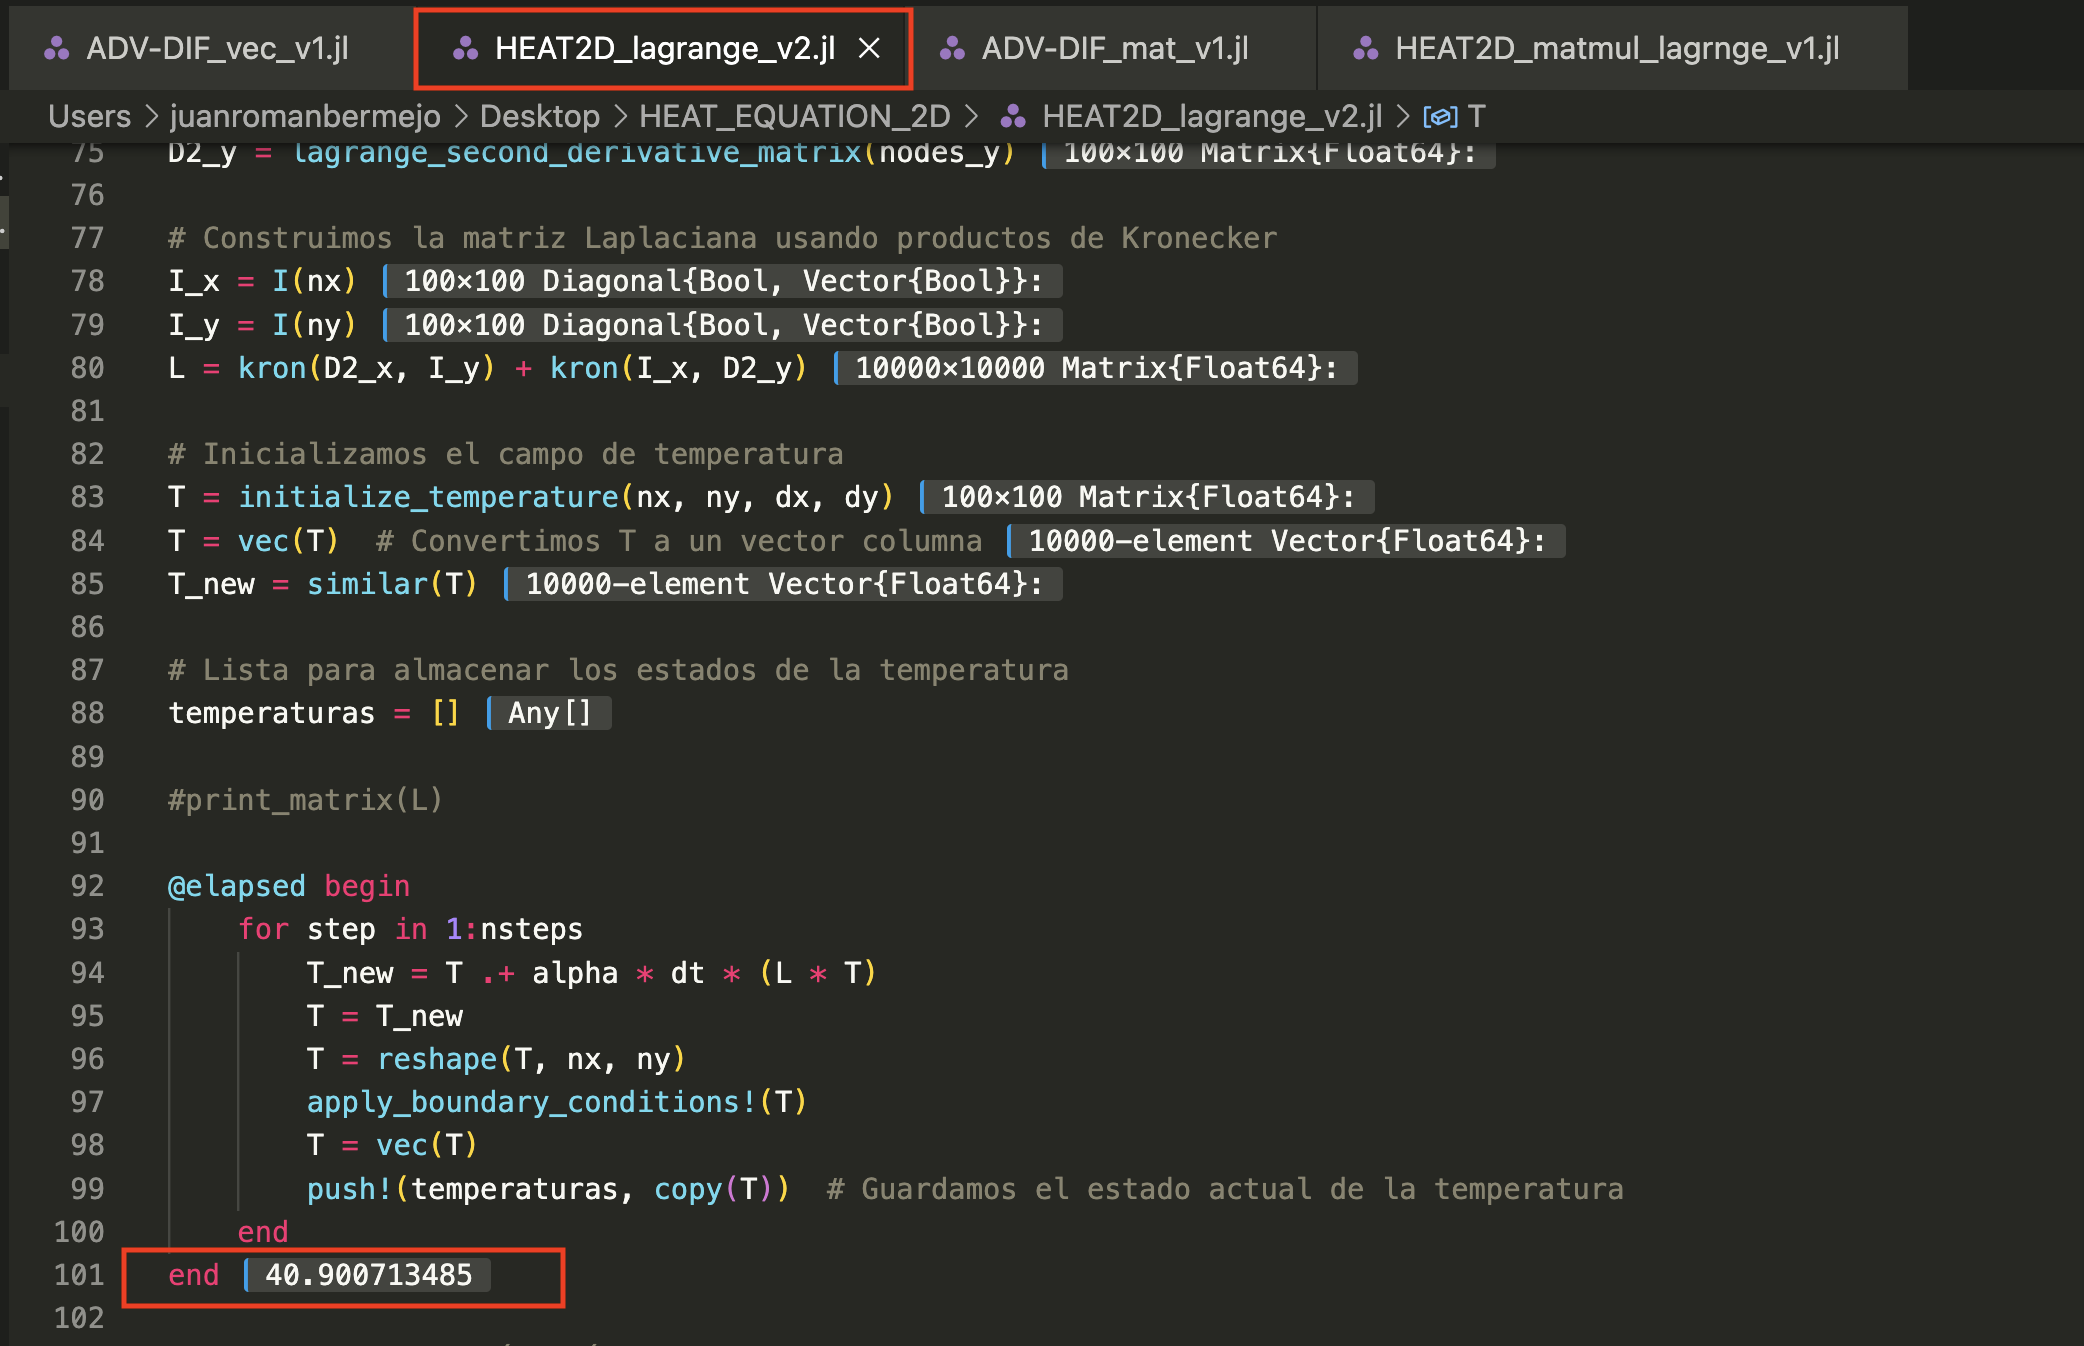
\includegraphics[width=0.7\textwidth]{Figures/HEAT-VEC-time.png}
    \caption{ Matrix-vector}
    \label{fig:etiqueta_figure}
\end{figure}


\begin{figure}[H]
    \centering
    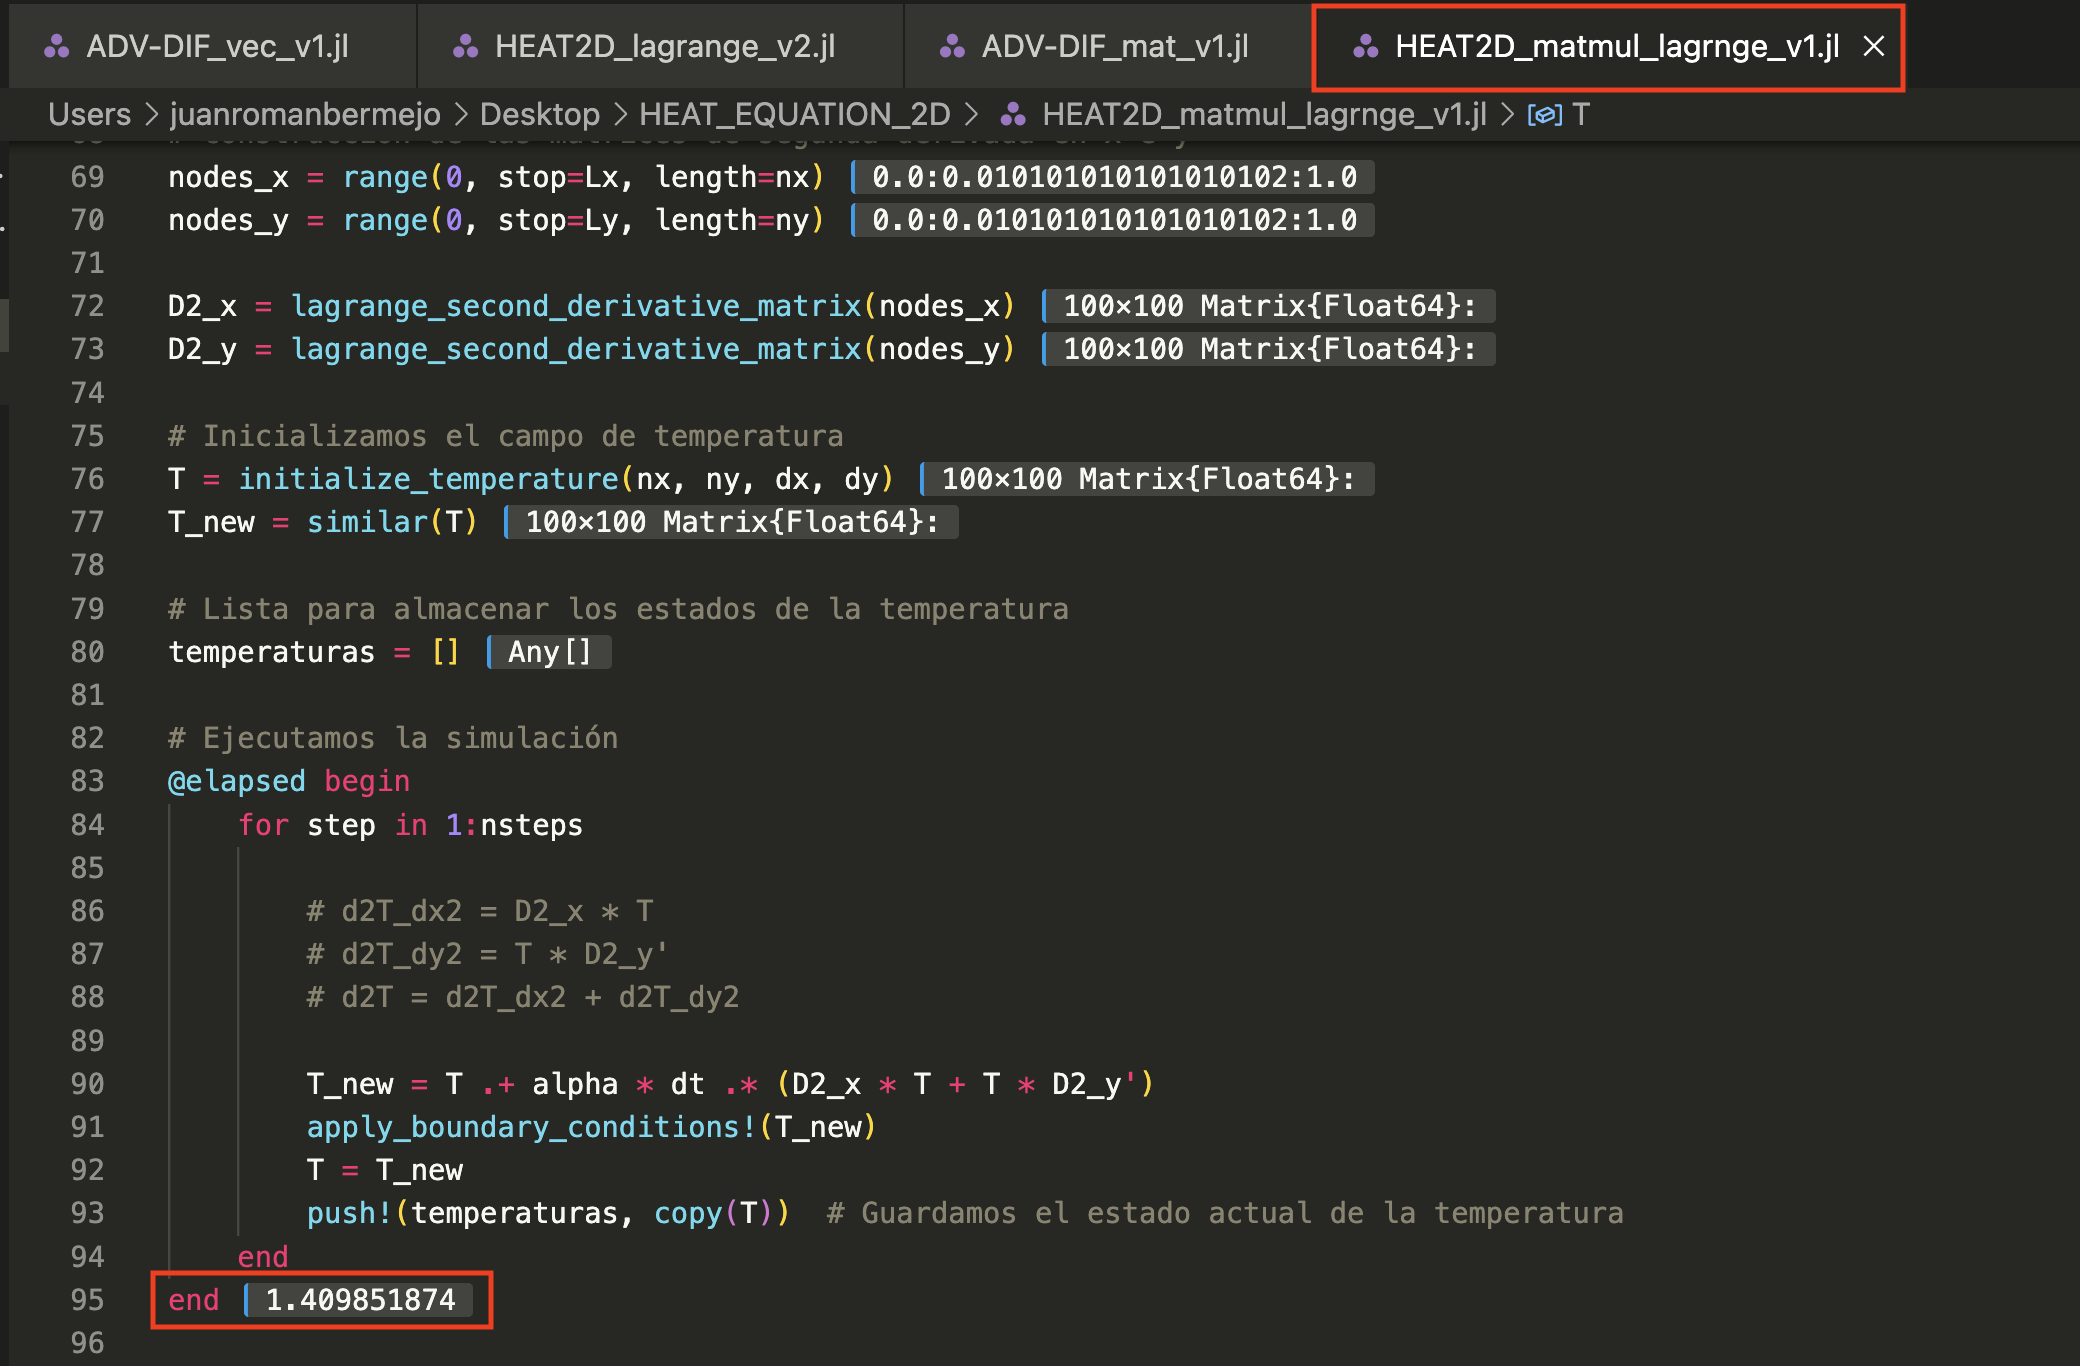
\includegraphics[width=0.7\textwidth]{Figures/HEAT-MAT-time.png}
    \caption{Matriz por Matriz}
    \label{fig:etiqueta_figure}
\end{figure}


\newpage
The results are the following: 


\begin{figure}[h!]
    \centering
    \begin{minipage}[b]{0.3\textwidth}
        \centering
        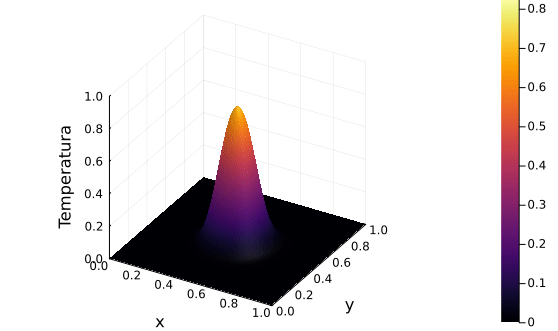
\includegraphics[width=\textwidth]{Figures/inicb.png}
        \caption{Image 1}
    \end{minipage}
    \hfill
    \begin{minipage}[b]{0.3\textwidth}
        \centering
        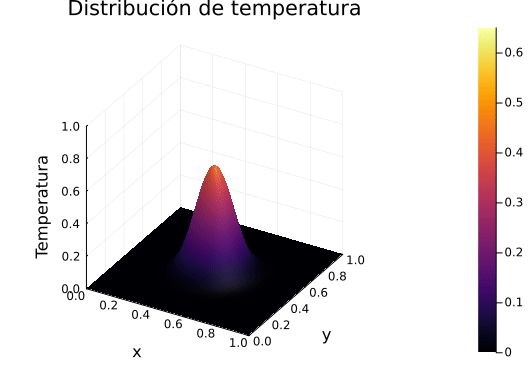
\includegraphics[width=\textwidth]{Figures/inic.png}
        \caption{Image 2}
    \end{minipage}
    \hfill
    \begin{minipage}[b]{0.3\textwidth}
        \centering
        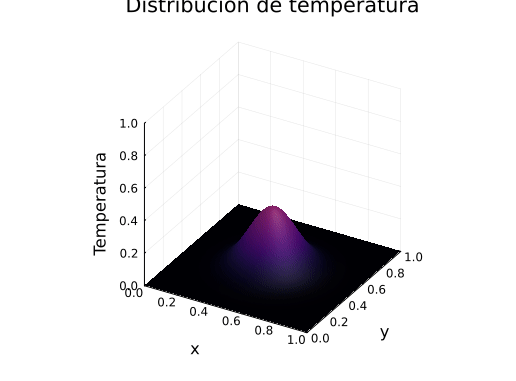
\includegraphics[width=\textwidth]{Figures/end.png}
        \caption{Image 3}
    \end{minipage}
\end{figure}



After these results, we attempted a more complex simulation, where we observed the evolution of the temperature around a rectangle at a constant temperature $T_{\text{const}}$, immersed in a flow with a different ambient temperature $T_{\infty}$ and a uniform velocity. The first test is done using finite differences, as shown in the figure below(t=0.416):


\begin{figure}[H]
    \centering
    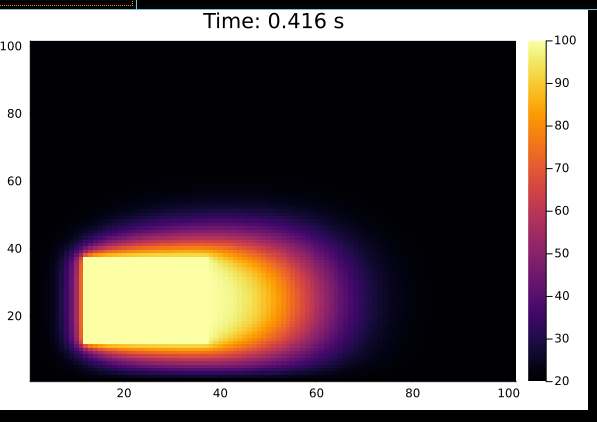
\includegraphics[width=0.7\textwidth]{Figures/rect2.png}
    \caption{Heat distribution around rectangle (t=0.416)}
    \label{fig:etiqueta_figure}
\end{figure}

\newpage 
The code used for this is the following:


\begin{lstlisting}[language=Julia]
using Plots
using Printf

# Parameters
nx, ny = 100, 100       # numero de puntos en x e y
Lx, Ly = 1.0, 1.0       # dimensiones del dominio
dx, dy = Lx/nx, Ly/ny   # espaciado de la malla
alpha = 0.01        # difusividad termica
T_inf = 20.0            # temperatura del aire entrante
T_rect = 100.0          # temperatura del rectangulo
u = 0.1            # velocidad del flujo de aire (izquierda a derecha)

# Esabilidad usando CFL 
dt_diff = (dx^2) / (2 * alpha)
dt_conv = dx / u
dt_max = min(dt_diff, dt_conv)
dt = min(dt_max, 0.0001)  # elegir dt estable

println("Paso temporal: $dt")
println("Maximo paso estable: $dt_max")

# Numero de pasos
t_end = 1.0             # tiempo final
nsteps = Int(t_end / dt)

# Inicializacion del campo de temperatura
T = fill(T_inf, nx+1, ny+1)

# Indices del rectangulo
rect_x = Int(floor(nx/8)):Int(floor(3*nx/8))
rect_y = Int(floor(ny/8)):Int(floor(3*ny/8))
T[rect_x, rect_y] .= T_rect

# Condiciones de contorno
function apply_boundary_conditions!(T, T_inf, u, dt, dx)
    nx, ny = size(T)
    
    # Inflow (left side)
    T[1, :] .= T_inf
    
    # Outflow (right side) - COND CONT Convectiva outflow 
   # for j in 1:ny
   #     T[end, j] = T[end, j] - u * dt / dx * (T[end, j] - T[end-1, j])
    #end
    
    



    # Arriba 
    T[:, end] .= T_inf
    
    # Abajo 
    T[:, 1] .= T_inf
end

# Actualizar el campo de temperatura
function update_temperature!(T, alpha, u, dx, dy, dt)
    nx, ny = size(T)
    T_new = copy(T)
    for i in 2:nx-1
        for j in 2:ny-1
            # Conveccion
            convection = -u * (T[i,j] - T[i-1,j]) / dx
 #upwinding
 
 # Tx = Dx T  Incluye todas las derivadas (cualquier orden) ver Matvect/ matmat// para ver comparacion(tiempo y resultados) u*gradT
            # Difusion

            # Txx = Dxx T igual evaluar que implementacion va mas rapido Dxx la calculas una vez 

            diffusion = alpha * (
                (T[i+1,j] - 2*T[i,j] + T[i-1,j]) / dx^2 +
                (T[i,j+1] - 2*T[i,j] + T[i,j-1]) / dy^2 )
            
            T_new[i,j] = T[i,j] + dt * (convection + diffusion)
        end
    end
    return T_new
end

# Temperatura del rectangulo
function set_rectangle_temperature!(T, rect_x, rect_y, T_rect)
    T[rect_x, rect_y] .= T_rect
end

# Configuracion de la visualizacion
anim = Animation()

# Bucle de integracion en el tiempo
for step in 1:nsteps
    # Aplicar condiciones de contorno
    apply_boundary_conditions!(T, T_inf, u, dt, dx)

    # Actualizar el campo de temperatura
    global T = update_temperature!(T, alpha, u, dx, dy, dt)

    # Fijar la temperatura del rectangulo
    set_rectangle_temperature!(T, rect_x, rect_y, T_rect)

    # Visualizacion
    if step % 10 == 0
        heatmap(T', c=:inferno, clim=(T_inf, T_rect), title=@sprintf("Time: %.3f s", step*dt))
        frame(anim)
    end
end

# Guardar la animacion como GIF
gif(anim, "heat_transfer_simulation1.gif", fps=10)

\end{lstlisting}

\clearpage
\subsection{Global Interpolation solving}

The next step is to solve the simulation using other methods that will allow us to compare 
implementations that perform matrix-vector operations to matrix-matrix operations.
The choice is to solve the equation using a Global Interpolation based on Lagrange polynomials, The Code used is listed below and performs matrix-matrix operations to solve the problem: 


\begin{lstlisting}[language=Julia]
#using Pkg
#Pkg.add("Plots")
#Pkg.add("Kronecker")
using LinearAlgebra, SparseArrays, Kronecker, BenchmarkTools
using Plots

function print_matrix(m)
    for row in 1:size(m, 1)
        println(join(m[row, :], " "))
    end
end

# Parametros del problema
nx = 25  # Numero de puntos en la direccion x
ny = 25   # Numero de puntos en la direccion y
Lx = 1.0  # Longitud del dominio en la direccion x
Ly = 1.0  # Longitud del dominio en la direccion y
alpha = 0.001  # Difusividad termica
v = [0, 0.01]  # Vector de velocidad (vx, vy)
dt = 0.01  # Paso de tiempo
tfinal = 15  # Tiempo final de la simulacion
nsteps = Int(tfinal / dt)  # Numero de pasos de tiempo

# Definimos el tamano de la malla
dx = Lx / (nx - 1)
dy = Ly / (ny - 1)

# Inicializacion continua de temperaturas
function initialize_temperature(nx, ny, dx, dy)
    T = zeros(nx, ny)
    for i in 1:nx
        for j in 1:ny
            x = (i-1) * dx
            y = (j-1) * dy
            T[i,j] = exp(-(25*(x-0.5)^2 + 25*(y-0.5)^2))
            if T[i,j] < 0
                T[i,j] = 0
            end
        end
    end
    return T
end



# Funcion para aplicar las condiciones de frontera y mantener la fuente termica fija
function apply_boundary_conditions!(T, nx, ny, dx, dy)
    # Mantener la temperatura fija en los bordes
    T[1, :] .= exp(-(25*(-0.5)^2))
    T[end, :] .= exp(-(25*(0.5)^2))
    T[:, 1] .= exp(-(25*(-0.5)^2))
    T[:, end] .= exp(-(25*(0.5)^2))

    # Mantener la fuente termica fija en el centro con la condicion inicial
    # for i in 1:nx
    #     for j in 1:ny
    #         x = (i-1) * dx
    #         y = (j-1) * dy
    #         distance = sqrt((x - 0.5)^2 + (y - 0.5)^2)
    #         if distance <= 0.05
    #             #T[i,j] = exp(-(25*(x-0.5)^2 + 25*(y-0.5)^2))
    #             T[i,j] = 1
    #         end
    #     end
    # end
end



# Definimos los nodos en x e y
nodes_x = range(0, stop=Lx, length=nx)
nodes_y = range(0, stop=Ly, length=ny)



# ======================================================================================================

# Calculo de los polinomios de Lagrange para los x
function lagrange_basis(x_nodes, i, x)
    l_i = 1.0
    for j in 1:length(x_nodes)
        if j != i
            l_i *= (x - x_nodes[j]) / (x_nodes[i] - x_nodes[j])
        end
    end
    return l_i
end

# Funcion para calcular la derivada del polinomio de Lagrange
function lagrange_derivative(x_nodes, i, x)
    dl_i = 0.0
    for m in 1:length(x_nodes)
        if m != i
            term = 1.0 / (x_nodes[i] - x_nodes[m])
            for j in 1:length(x_nodes)
                if j != i && j != m
                    term *= (x - x_nodes[j]) / (x_nodes[i] - x_nodes[j])
                end
            end
            dl_i += term
        end
    end
    return dl_i
end

# Funcion para calcular la matriz de derivadas usando polinomios de Lagrange
function lagrange_derivative_matrix(x_nodes)
    n = length(x_nodes)
    D = zeros(n, n)
    for i in 1:n
        for j in 1:n
            D[i, j] = lagrange_derivative(x_nodes, j, x_nodes[i])
        end
    end
    return D
end


# Definimos los nodos en x e y
nodes_x = range(0, stop=Lx, length=nx)
nodes_y = range(0, stop=Ly, length=ny)

# Construccion de las matrices de derivadas con POLINOMIOS DE LAGRANGE
D_x = lagrange_derivative_matrix(nodes_x)
D_y = lagrange_derivative_matrix(nodes_y)

# Las matrices de segunda derivada son simplemente el producto de la matriz de primera derivada con ella misma
D2_x = D_x * D_x
D2_y = D_y * D_y

# ============================================================================================================




# Inicializamos el campo de temperatura
T = initialize_temperature(nx, ny, dx, dy)  # Convertimos T a un vector columna
T_new = similar(T)

# Lista para almacenar los estados de la temperatura
temperaturas = []


# Medir el tiempo del bucle
@elapsed begin
    for step in 1:nsteps

        # difusion = alpha * (Laplacian * T)
        # adveccion = -(Gradient * T)

        T_new = T .+ dt .* (alpha * (D2_x * T + T * D2_y') - (v[1] * (D_x * T) + v[2] * (T * D_y')))
        
        global T = T_new
        apply_boundary_conditions!(T, nx, ny, dx, dy)
        push!(temperaturas, copy(T))  # Guardamos el estado actual de la temperatura
    end
end


## === REPRESENTACION GRAFICA === ##

# Convertimos el resultado a una matriz para mostrarlo
T = reshape(T, nx, ny)

# Determinamos los limites de los ejes
x = range(0, stop=Lx, length=nx)
y = range(0, stop=Ly, length=ny)
z_min, z_max = 0, 1.0  # Limites del eje z (temperatura)

# # Creamos la animacion 3D
# intervalo_animacion = 30
# animation = @animate for i in 1:intervalo_animacion:length(temperaturas)
#     t = temperaturas[i]
#     surface(x, y, reshape(t, nx, ny), title="Distribucion de temperatura [M][M]", xlabel="x", ylabel="y", zlabel="Temperatura", c=:inferno, xlims=(0, Lx), ylims=(0, Ly), zlims=(z_min, z_max))
# end

# # Guardamos la animacion como un gif
# gif(animation, "adveccion_difusion_diferencias_finitas_matxmat_3d.gif", fps=30)


# Creamos la animacion 2D con lineas de contorno sin letras
intervalo_animacion = 30
animation = @animate for i in 1:intervalo_animacion:length(temperaturas)
    t = temperaturas[i]
    contourf(x, y, reshape(t, nx, ny), c=:inferno, xlims=(0, Lx), ylims=(0, Ly), zlims=(z_min, z_max), xlabel="", ylabel="", title="", clabels=false)
end

# Guardamos la animacion como un gif
gif(animation, "adveccion_difusion_contornos2d.gif", fps=10)
\end{lstlisting}

Now with a matrix-vector approach:



\subsubsection*{1. Heat Diffusion}
The heat diffusion equation describes how heat spreads through the medium over time due to thermal diffusivity. Mathematically, it is expressed as:

\[
\frac{\partial T}{\partial t} = \alpha \left( \frac{\partial^2 T}{\partial x^2} + \frac{\partial^2 T}{\partial y^2} \right)
\]

where:
\begin{itemize}
    \item \( T(x, y, t) \) is the temperature field,
    \item \( \alpha \) is the thermal diffusivity, which determines the rate at which heat diffuses through the material,
    \item \( \frac{\partial^2 T}{\partial x^2} \) and \( \frac{\partial^2 T}{\partial y^2} \) are second-order spatial derivatives representing the diffusion of heat in the \( x \) and \( y \) directions.
\end{itemize}

In this simulation, the diffusion term is discretized using \textbf{Lagrange polynomial interpolation} to approximate the second-order derivatives in both directions.
\newpage
\subsubsection*{2. Advection}
Advection describes the transport of heat due to fluid motion, which can be represented as:

\[
-\mathbf{v} \cdot \nabla T = -v_x \frac{\partial T}{\partial x} - v_y \frac{\partial T}{\partial y}
\]

where:
\begin{itemize}
    \item \( \mathbf{v} = (v_x, v_y) \) is the velocity field, representing the movement of the heat due to fluid flow,
    \item \( \nabla T \) is the gradient of the temperature, representing the directional change in temperature.
\end{itemize}

In this simulation, the velocity vector \( \mathbf{v} = [0, 0.01] \) causes heat to be advected primarily in the \( y \)-direction (upward).

\subsubsection*{3. Initial and Boundary Conditions}
\begin{itemize}
    \item \textbf{Initial Condition:} The temperature field is initialized with a Gaussian-like heat distribution centered at the middle of the domain. This represents a concentrated heat source that spreads out over time.
    \item \textbf{Boundary Conditions:} The domain has fixed temperature values at its boundaries (Dirichlet conditions). These remain constant throughout the simulation, enforcing a specific temperature on the edges of the domain.
\end{itemize}

\subsubsection*{4. Numerical Method}
The simulation uses \textbf{Lagrange polynomials} to discretize the spatial derivatives in both the \( x \)- and \( y \)-directions. This allows us to approximate the spatial derivatives necessary for solving the heat equation. 

At each time step, the temperature field is updated using the following equation:

\[
T_{\text{new}} = T + \Delta t \left( \alpha \left( \frac{\partial^2 T}{\partial x^2} + \frac{\partial^2 T}{\partial y^2} \right) - v_x \frac{\partial T}{\partial x} - v_y \frac{\partial T}{\partial y} \right)
\]

where \( \Delta t \) is the time step size, \( \alpha \) controls the rate of heat diffusion, and \( v_x \) and \( v_y \) represent the velocities in the \( x \)- and \( y \)-directions (advection).
\newpage
\subsubsection*{5. Visualization}
The simulation results are visualized as contour plots, which show the evolving temperature field over time. The animation demonstrates how the heat diffuses across the domain while being transported upward by the advection process.

\subsubsection*{Key Physical Concepts}
\begin{itemize}
    \item \textbf{Heat Diffusion:} The process by which heat spreads from areas of high temperature to low temperature.
    \item \textbf{Advection:} The transport of heat due to the fluid motion, represented by the velocity vector \( \mathbf{v} \).
    \item \textbf{Lagrange Polynomial Interpolation:} Used to discretize the spatial derivatives of the temperature field.
    \item \textbf{Boundary Conditions:} Fixed temperature values are enforced on the domain boundaries.
\end{itemize}

This combination of heat diffusion and advection captures the behavior of heat flow in systems with fluid motion and thermal effects. The numerical method used here allows for the accurate simulation of temperature evolution in the domain.

\begin{figure}[h!]
    \centering
    \begin{minipage}[b]{0.3\textwidth}
        \centering
        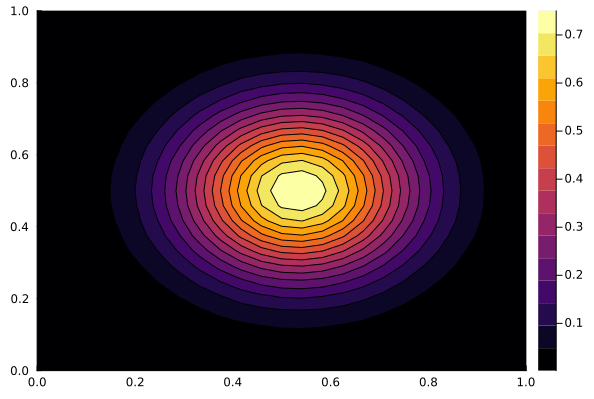
\includegraphics[width=\textwidth]{Figures/CD1.png}
        \caption{$t = 0\,\text{s}$}
    \end{minipage}
    \hfill
    \begin{minipage}[b]{0.3\textwidth}
        \centering
        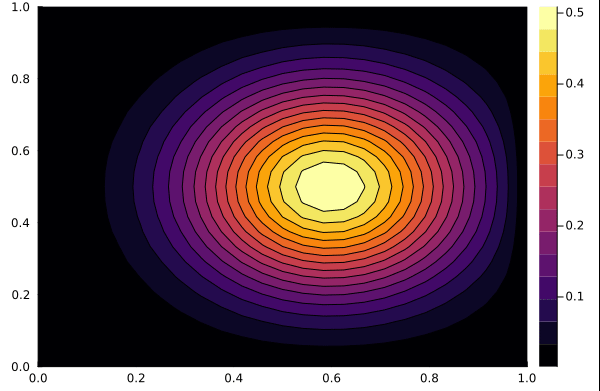
\includegraphics[width=\textwidth]{Figures/CD2.png}
        \caption{$t = 7.5\,\text{s}$}
    \end{minipage}
    \hfill
    \begin{minipage}[b]{0.3\textwidth}
        \centering
        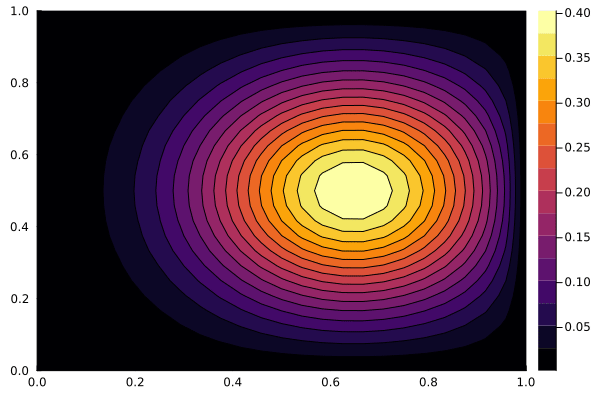
\includegraphics[width=\textwidth]{Figures/CD3.png}
        \caption{$t = 15\,\text{s}$}
    \end{minipage}
\end{figure}


\clearpage
\paragraph{Extra comparison}

As an extra step, this code written by Javier solves the equation in 1D, 2D, or 3D , we will compare it to the other results 



\begin{lstlisting}[language=Julia]
using LinearAlgebra, GLMakie


function heatpropagate(u::AbstractArray{T,N}, timesteps::Integer, αΔtΔx⁻²::Real,
    uprev::AbstractArray{T,N}) where {T<:Number,N}

    αΔtΔx⁻² ≤ 0.5 / N || throw(ArgumentError("αΔtΔx⁻² = $αΔtΔx⁻² violates Fourier stability condition"))

    unitvecs = ntuple(i -> CartesianIndex(ntuple(==(i), Val(N))), Val(N))

    I = CartesianIndices(u)
    Ifirst, Ilast = first(I), last(I)
    I1 = oneunit(Ifirst)

    for t = 1:timesteps

        @inbounds @simd for i in Ifirst+I1:Ilast-I1

            ∇²u = -2N * u[i]
            for uvec in unitvecs
                ∇²u += u[i+uvec] + u[i-uvec]
            end

            u[i] = uprev[i] + αΔtΔx⁻² * ∇²u

        end

        # Here Boundary conditions would be imposed (except if they are Dirichlet at boundary)

        uprev = u
    end

    return u, uprev
end

begin
    x = range(-1.0, 1.0, length=100)
    u = @. exp(-(x / 0.2)^2)
    u[1] = u[end] = 0.0

    set_publication_theme!()

    lines(x, u)

    α = 1.0
    Δx = x[2] - x[1]
    Fo = 1 / 2
    Δt = Fo * Δx^2 / α

    uprev = copy(u)
end

# @time heatpropagate(u, 20, Fo, uprev);

for i = 1:50
    u, uprev = heatpropagate(u, 20, Fo, uprev)
    lines!(x, u)
end

\end{lstlisting}



\subsubsection{Graphs and tables}

 Graphs and tables summarizing the results obtained, allowing a comparison between the different methods and/or hardware platforms.






\begin{table}[h!]
\centering
\begin{tabular}{|c|c|}
\hline
\textbf{Method} & \textbf{Simulation Time (seconds)} \\ \hline
Global Interpolant (matrix-matrix) &  0.127 \\ \hline
Global Interpolant (matrix-vector) &  2.789   \\ \hline
Finite Differences & 0.646 \\ \hline
Javier`s Code & ?? \\ \hline
\end{tabular}
\caption{Comparison of methods and expected simulation times}
\label{table:methods_time}
\end{table}








\clearpage

\subsection{Conclusions}

This study researches different numerical methods to solve the heat equation with convective and diffusive terms. The aim is to compare the different approaches and verify that the theoretical hypothesis are approximately proven. 


clearpage

\subsection{Bibliografía}

\begin{itemize}
    \item Juan A. Hernandez Ramos 
Mario A. Zamecnik Barros. \textit{Interpolación Polinómica de Alto orden, Métodos Espectrales}
    \item Smith, G. D. (1985). \textit{Numerical Solution of Partial Differential Equations: Finite Difference Methods}. Oxford University Press.
    \item LeVeque, R. J. (2007). \textit{Finite Difference Methods for Ordinary and Partial Differential Equations: Steady-State and Time-Dependent Problems}. Society for Industrial and Applied Mathematics.
    \item Kirk, D. B., \& Hwu, W.-m. W. (2016). \textit{Programming Massively Parallel Processors: A Hands-on Approach}. Morgan Kaufmann.
    \item Román Bermejo, J. (2024). \textit{CPU Performance: Benchmark Analysis and Theoretical Limits}.
    \item{Boyd2001}
J. P. Boyd. (2001)\textit{Chebyshev and Fourier Spectral Methods}, 2nd edition, Dover Publications.

 
\end{itemize}






\clearpage


%   ---   BIBLIOGRAFÍA/REFERENCIAS   ---   %

%\phantomsection
%\addcontentsline{toc}{section}{Referencias}
%\renewcommand{\refname}{Referencias}
%\bibliographystyle{elsarticle-num}
%\bibliography{references.bib}
%\clearpage



%   ---   ANEXOS   ---   %

%\appendix
%\renewcommand{\appendixname}{Anexos}
%\addcontentsline{toc}{section}{\appendixname}
%\clearpage % or \cleardoublepage
%\appendixpage
%\addappheadtotoc
%\renewcommand{\appendixname}{Anexo}


%\input{./Tex_Files/A_01.tex}
%\clearpage

\end{document}